\chapter{Generating random performance tableaux}
\label{sec:6}

\abstract*{ The chapter describes the \Digraph \texttt{randomPerfTabs} module for generating random multiple criteria performance tableaux. The module proposes several useful models, like a \emph{Cost-Benefit} tableau, a three Objectives --\emph{economic}, \emph{societal} and \emph{environmental}-- tableau, and an \emph{academic} performance tableau.} 

\abstract{ The chapter describes the \Digraph \texttt{randomPerfTabs} module for generating random multiple criteria performance tableaux. The module proposes several useful random models, like a \emph{Cost-Benefit} tableau, a three Objectives --\emph{economic}, \emph{societal} and \emph{environmental}-- tableau, and an \emph{academic} performance tableau.}

\section{Introduction}
\label{sec:6.1}

The \texttt{randomPerfTabs} module provides several classes for generating random performance tableaux models of different kind, mainly for the purpose of testing implemented methods and tools presented and discussed in the Algorithmic Decision Theory course lectures at the University of Luxembourg. This chapter introduces the most useful models.

The simplest generic class, called \texttt{RandomPerformanceTableau}, generates a set of $n$ decision actions, a family of $m$ real-valued performance criteria, ranging by default from $0.0$ to $100.0$, associated with default discrimination thresholds: $2.5$ (ind.), $5.0$ (pref.) and $60.0$ (veto). The generated random grades are by default \texttt{Beta(2,2)} distributed on each measurement scale.

One of the most useful models, called \texttt{RandomCBPerformanceTableau}\index{}, proposes a performance tableau involving two decision objectives, named \emph{Costs} (to be minimised) respectively \emph{Benefits} (to be maximised); its purpose being to generate more or less contradictory performances on these two, usually conflicting, objectives. \emph{Low costs} will randomly be correlated with \emph{low benefits}, whereas \emph{high costs} will randomly be correlated with \emph{high benefits}.

Many public policy decision problems involve three often conflicting decision objectives taking into account \emph{economical}, \emph{societal} as well as \emph{environmental} aspects. For this type of performance tableau model, we provide a specific model, called \texttt{Random3ObjectivesPerformanceTableau}.

Deciding which students, based on the grades obtained in a number of examinations, validate or not their academic studies, is the genuine decision practice of universities and academies. To thoroughly study these kind of decision problems, we provide a corresponding performance tableau model, called \texttt{RandomAcademic\-PerformanceTableau}, which gathers grades obtained by a given number of students in a given number of weighted courses.    

In order to study aggregation of election results (see Chapter~\vref{sec:7}) in the context of bipolar-valued outranking digraphs, we provide furthermore a specific performance tableau model called \texttt{RandomRankPerformanceTableau} which provides ranks (linearly ordered performances without ties) of a given number of election candidates (decision actions) for a given number of weighted voters (performance criteria).
 
\section{Random standard performance tableaux}
\label{sec:6.2}
    
The \texttt{RandomPerformanceTableau} class\index{RandomPerformanceTableau@\texttt{RandomPerformanceTableau} class}, the simplest of the kind, specializes the generic \texttt{PerformanceTableau} class, and takes the following parameters:
\begin{itemize}[leftmargin=0.5cm,rightmargin=0.5cm]
\item \texttt{numberOfActions} := number of decision actions.
\item \texttt{numberOfCriteria} := number of performance criteria.
\item \texttt{weightDistribution} := \\
   \texttt{'random'} (default) $|$ \texttt{'fixed'} $|$ \texttt{'equisignificant'}:
      \begin{itemize}[rightmargin=1cm,topsep=1pt]
         \item If \texttt{'random'}, weights are uniformly selected randomly from the given weight scale;
         \item If \texttt{'fixed'}, the weightScale must provided a corresponding weights distribution;
         \item If \texttt{'equi-significant'}, all criterion weights are put to unity.
      \end{itemize}
\item \texttt{weightScale} := \texttt{[Min,Max]} (default =(1, \texttt{numberOfCriteria}).
\item \texttt{IntegerWeights} := \texttt{True} (default) $|$ \texttt{False} (normalised to proportions of $1.0$).
\item \texttt{commonScale} := \texttt{[a,b]}; common performance measuring scales (default = $[0.0,100.0]$)
\item \texttt{commonThresholds} := [(\texttt{q0}, \texttt{q1}), (\texttt{p0}, \texttt{p1}), (\texttt{v0}, \texttt{v1})]; indifference($q$), preference ($p$) and considerable performance difference ($v$) discrimination thresholds. For each threshold type $x \in \{q,p,v\}$, the float $x0$ value represents a \emph{constant percentage} of the common scale and the float $x1$ value a \emph{proportional value} of the actual performance measure. Default values are $[(2.5.0,0.0), (5.0,0.0), (60.0,0,0)]$. 
\item \texttt{commonMode} := common distribution of random performance measurements\footnote{See Lecture 3 of the Computational Statistic Course \citep{CPSTAT-L3}.}:
      \begin{itemize}[rightmargin=1cm]
         \item (\texttt{'beta'}, \texttt{None} (default setting), ($\alpha$, $\beta$)), a beta generator with default $\alpha=2$ and $\beta=2$ parameters.
         \item  (\texttt{'uniform'}, \texttt{None}, \texttt{None}), uniformly distributed float values on the given common scales' range \texttt{[Min, Max]};
         \item (\texttt{'normal'}, $\mu$, $\sigma$), truncated Gaussian distribution, by default $\mu = (b-a)/2$ and $\sigma = (b-a)/4$;
         \item (\texttt{'triangular'}, \emph{mode}, \emph{repartition}), generalised triangular distribution with a probability repartition parameter specifying the probability mass accumulated until the mode value. By default, \emph{mode} = $(b-a)/2$ and \texttt{repartition} = $0.5$.\footnote{The \texttt{randomNumbers}\index{randomNumbers@\texttt{randomNumbers} module} module provides for this purpose the \texttt{ExtendedTriangularRandomVariable} class\index{ExtendedTriangularRandomVariable@\texttt{ExtendedTriangularRandomVariable} class}.}
      \end{itemize}
\item \texttt{valueDigits} := \texttt{integer}, precision of performance measurements (2 decimal digits by default).
\item \texttt{missingDataProbability} := $0.0 \leq \mathtt{float} \leq 1.0$ ; probability of missing performance evaluation on a criterion for an alternative (default $0.025$).
\item \texttt{NA} := \texttt{Decimal} (default = $-999$); missing data symbol. \end{itemize} 

\noindent \textbf{Code example:}
\begin{lstlisting}[caption={Generating a random performance tableau},label=list:6.1]
>>> from randomPerfTabs import RandomPerformanceTableau
>>> t = RandomPerformanceTableau(numberOfActions=21,\
...                 numberOfCriteria=13,seed=100)
>>> t.actions
  {'a01': {
    'comment': 'RandomPerformanceTableau() generated.',
    'name': 'random decision action'
    },
   'a02': { ... },
    ...
   }
>>> t.criteria
  {'g01': {
    'thresholds': {
      'ind' : (Decimal('10.0'), Decimal('0.0')),
      'veto': (Decimal('80.0'), Decimal('0.0')),
      'pref': (Decimal('20.0'), Decimal('0.0'))},
    'scale': [0.0, 100.0],
    'weight': Decimal('1'),
    'name': 'RandomPerformanceTableau() instance',
    'comment': "Arguments: weightDistribution=random;
                           weightScale=(1, 1);
                           commonMode=None"
    },
   'g02':  { ... },
   ...
 }
>>> t.NA
  Decimal('-999')
>>> t.evaluation
  {'g01': {'a01': Decimal('15.17'),
           'a02': Decimal('44.51'),
           'a03': Decimal('-999'), # missing evaluation
       ...  },
   ...
 }
>>> t.showHTMLPerformanceTableau()
\end{lstlisting}
\begin{figure}[ht]
%\sidecaption
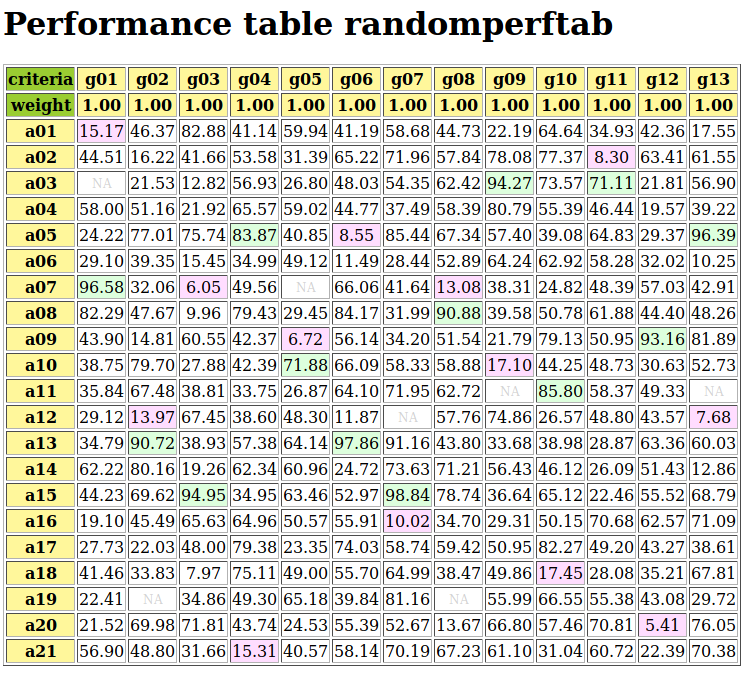
\includegraphics[width=\hsize]{Figures/6-1-randomPerfTab1.png}
\caption{Browser view on random performance tableau instance}
\label{fig:6.1}       % Give a unique label
\end{figure}

Best and worst performance on each criterion are marked in \emph{light green}, respectively in \emph{light red}. Notice that missing (\texttt{NA}) evaluation are registered in a performance tableau by default as \texttt{Decimal('-999')} value (see Listing~\vref{list:6.1} Line 28-29).	    

\section{Random Cost-Benefit performance tableaux}
\label{sec:6.3}

The \texttt{randomPerfTabs} module provides a \texttt{RandomCBPerformanceTableau} class\index{RandomCBPerformanceTableau@\texttt{RandomCBPerformanceTableau} class} for generating random \emph{Costs} versus \emph{Benefits} organised performance tableaux. The random generator is following the directives below:
\begin{itemize}[leftmargin=0.5cm,rightmargin=0.25cm]
\item Three types of decision actions are distinguished: \emph{cheap}, \emph{neutral} and \emph{expensive} ones with an equal proportion of 1/3. Two types of weighted criteria are also distinguished: \emph{Costs} criteria to be \emph{minimised}, and \emph{Benefits} criteria to be \emph{maximised}, in the proportions 1/3 respectively 2/3;
\item  Random performances on each type of criteria  are drawn, either from an ordinal scale $[0;10]$, or from a cardinal scale $[0.0;100.0]$, following a parametric triangular law of mode: $30\%$ performance for cheap, $50\%$ for neutral, and $70\%$ performance for expensive decision actions, with constant probability repartition $0.5$ on each side of the respective mode;
\item Costs criteria use mostly cardinal scales (3/4), whereas Benefits criteria use mostly ordinal scales (2/3); 
\item  The sum of weights of the Costs criteria equals by default the sum of weights of the Benefits criteria: \texttt{weighDistribution = 'equiobjectives'};
\item On cardinal criteria, both of cost or of benefit type, following constant performance discrimination quantiles are instantiated: $5\%$ indifferent situations, $90\%$ preference situations, and $5\%$ considerable performance difference situations. 
\end{itemize}

\noindent \textbf{Parameters}:
\begin{itemize}[leftmargin=0.5cm,rightmargin=0.5cm]
\item If \texttt{numberOfActions == None}, a uniform random number between 10 and 31 of \emph{cheap}, \emph{neutral} or \emph{advantageous} actions (equal 1/3 probability each type) actions is instantiated. Minimal number of decision actions required is 3; 
 \item If \texttt{numberOfCriteria == None}, a uniform random number between 5 and 21 of cost or benefit criteria (1/3 respectively 2/3 probability) is instantiated;
\item \texttt{weightDistribution} :=  \texttt{'equisignificant'} (default) $|$
 \texttt{'equi\-objectives'} $|$ \texttt{'fixed'} $|$ \texttt{'random'};
\item default \texttt{weightScale} for \texttt{'random'} weight distribution is 1 - \texttt{number\-OfCriteria};
\item All \emph{cardinal} criteria are evaluated with decimals between $0.0$ and $100.0$ whereas \emph{ordinal} criteria are evaluated with integers between 0 and 10.
\item \texttt{commonThresholds} is obsolete. Preference discrimination is specified as \emph{percentiles} of concerned performance differences (see below).
\item \texttt{commonPercentiles} := \texttt{\{'ind':5, 'pref':10, 'veto':95\}} are expressed in percents (reversed for vetoes), and only concern cardinal criteria.
\item \texttt{missingDataProbability} := $0.0 \leq \mathtt{float} \leq 1.0$ ; probability of missing performance evaluation on a criterion for an alternative (default $0.025$).
\item \texttt{NA} := \texttt{Decimal} (default = $-999$); missing data symbol. 
\end{itemize}

\noindent \textbf{Example Python session}:
\begin{lstlisting}[caption={Generating a random Cost-Benefit performance tableau},label=list:6.2]
>>> from randomPerfTabs import\
...              RandomCBPerformanceTableau
>>> t = RandomCBPerformanceTableau(
...          numberOfActions=7,\
...          numberOfCriteria=5,\
...          weightDistribution='equiobjectives',\
...          commonPercentiles={'ind':0.05,
...                             'pref':0.10,\
                                'veto':0.95},\
...          seed=100)
>>> t.showActions()
  *----- show decision action --------------*
    key:  a1
      short name: a1c
      name:  random cheap decision action
    key:  a2
      short name: a2n
      name:  random neutral decision action
    ...
    key:  a7
      short name: a7a
      name:  random advantageous decision action
>>> t.showCriteria()
  *----  criteria -----*
   b1 'random ordinal benefit criterion'
    Preference direction: max
    Scale = (0, 10)
    Weight = 3
    ...
   c1 'random cardinal cost criterion'
    Preference direction: min
    Scale = (0.0, 100.0)
    Weight = 2 
    Threshold ind  :  1.76 + 0.00x ; percentile:  9.5
    Threshold pref :  2.16 + 0.00x ; percentile: 14.3
    Threshold veto : 73.19 + 0.00x ; percentile: 95.2
    ...}
\end{lstlisting}

In Listing~\vref{list:6.2} one may notice the three types of decision actions (see Lines 12-22), as well as the two types (Lines 24-35) of criteria with either an \emph{ordinal} or a \emph{cardinal} performance measuring scale. In the latter case, by default about $5\%$ of the random performance differences will be below the \emph{indifference} and $10\%$ below the \emph{preference} discriminating threshold. About $5\%$ will be \emph{considerably large}. More statistics about the generated performance grades may be inspected with the \texttt{showStatistics()} method.\index{showStatistics@\texttt{showStatistics()}}
\begin{lstlisting}
>>> t.showStatistics()
    *-------- Performance tableau summary statistics -------*
    Instance name      : randomCBperftab
    Actions            : 7
    Criteria           : 5
     Criterion name       : b1
       Criterion weight     : 3
       criterion scale    : 0.00 - 10.00
       mean evaluation    : 5.14
       standard deviation : 2.64
       maximal evaluation : 8.00
       quantile Q3 (x_75) : 8.00
       median evaluation  : 6.50
       quantile Q1 (x_25) : 3.50
       minimal evaluation : 1.00
       mean absolute difference      : 2.94
       standard difference deviation : 3.74
      ...
     Criterion name       : c1
       Criterion weight     : 2
       criterion scale    : -100.00 - 0.00
       mean evaluation    : -49.32
       standard deviation : 27.59
       maximal evaluation : 0.00
       quantile Q3 (x_75) : -27.51
       median evaluation  : -35.98
       quantile Q1 (x_25) : -54.02
       minimal evaluation : -91.87
       mean absolute difference      : 28.72
       standard difference deviation : 39.02
     ...
\end{lstlisting}

A heatmap view with 5 color levels gives the result shown in Fig.~\vref{fig:6.2}.
\begin{lstlisting}
>>> t.showHTMLPerformanceHeatmap(colorLevels=5,\
...        rankingRule=None,\
...        pageTitle='Random Cost-Benefit Performance Tableau')
 \end{lstlisting}
\begin{figure}[ht]
%\sidecaption
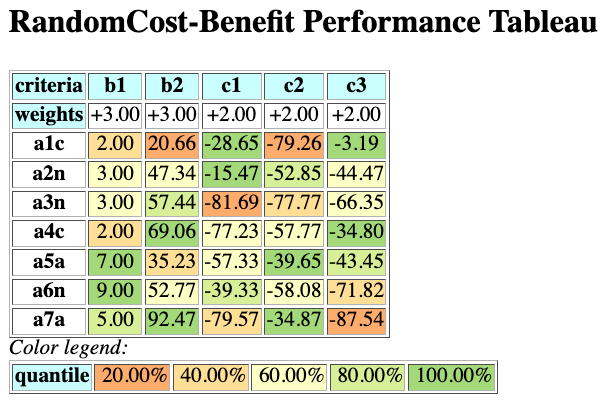
\includegraphics[width=10cm]{Figures/6-2-randomCBHeatmap.png}
\caption{Unordered heatmap of a random Cost-Benefit performance tableau}
\label{fig:6.2}       % Give a unique label
\end{figure}
 
Such a performance tableau may be stored and re-accessed as follows.
\begin{lstlisting}
>>> t.save('temp')
    *----- saving performance tableau in XMCDA 2.0 format  -------------*
    File: temp.py saved !
>>> from perfTabs import PerformanceTableau
>>> t = PerformanceTableau('temp')
\end{lstlisting}

\section{Random three objectives performance tableaux}
\label{sec:6.4}

The randomPerfTabs module provides a \texttt{Random3ObjectivesPerformance\-Tableau} class\index{Random3ObjectivesPerformanceTableau@\texttt{Random3ObjectivesPerformanceTableau} class} for generating random performance tableaux concerning public policies evaluated with respect to three decision objectives taking respectively into account \emph{economical}, \emph{societal} as well as \emph{environmental} aspects. Each potential public policy is qualified randomly as performing \emph{weak} ($-$), \emph{fair} ($\sim$) or \emph{good} ($+$) wrt to each one of the three objectives. 

\noindent \textbf{Generator directives are the following:}

\begin{itemize}[leftmargin=0.5cm,rightmargin=0.5cm]
\item \texttt{numberOfActions} = $20$ (default), minimal number required is 3; 
\item \texttt{numberOfCriteria} = $13$ (default),
\item \texttt{weightDistribution} = \texttt{'equiobjectives'} (default) $|$ \texttt{'random'} $|$ \texttt{'equisignificant'},
\item \texttt{weightScale} = (1,\texttt{numberOfCriteria}): only used when random criterion weights are requested,
\item \texttt{integerWeights} = \texttt{True} (default): \texttt{False} gives normalised rational weights, 
\item \texttt{commonScale} = ($0.0$,$100.0$),
\item \texttt{commonThresholds} = [$(5.0,0.0)$, $(10.0,0.0)$, $(60.0,0.0)$]: Performance discrimination thresholds may be set for \texttt{'ind'}, \texttt{'pref'} and \texttt{'veto'} thresholds,  
\item \texttt{commonMode} = [\texttt{'triangular'},\texttt{'variable'},$0.5$]: random number generators of various other types ('\emph{uniform}','\emph{beta}') are available. If the mode of the \texttt{'triangular'} distribution is set to \texttt{'variable'}, three modes at $0.3 (-)$, $0.5 (\sim)$, respectively $0.7 (+)$ of the common scale span are set at random for each coalition and action. 
\item \texttt{valueDigits} = 2 (default): evaluations are encoded as decimals,
\item \texttt{missingDataProbability} = $0.05$ (default): random insertion of missing values with given probability,  
\item \texttt{NA} := \texttt{Decimal} (default = $-999$); missing data symbol,
\item \texttt{seed} = \texttt{None} (default). 
\end{itemize}

\noindent \textbf{Example Python session:}
\begin{lstlisting}[caption={Generating a random 3 Objectives performance tableau},label=list:6.3]
>>> from randomPerfTabs import\
...            Random3ObjectivesPerformanceTableau
>>> t = Random3ObjectivesPerformanceTableau(\
...           numberOfActions=7,\
...           numberOfCriteria=13,\
...           weightDistribution='equiobjectives',\
...           seed=120)
>>> t.showObjectives()
  *------ show objectives -------"
   Eco: Economical aspect
    ec01 criterion of objective Eco 18
    ec05 criterion of objective Eco 18
    ec06 criterion of objective Eco 18
    ec12 criterion of objective Eco 18
    Total weight: 72.00 (4 criteria)
   Soc: Societal aspect
    so02 criterion of objective Soc 24
    so11 criterion of objective Soc 24
    so13 criterion of objective Soc 24
    Total weight: 72.00 (3 criteria)
   Env: Environmental aspect
    en03 criterion of objective Env 12
    en04 criterion of objective Env 12
    en07 criterion of objective Env 12
    en08 criterion of objective Env 12
    en09 criterion of objective Env 12
    en10 criterion of objective Env 12
    Total weight: 72.00 (6 criteria)
\end{lstlisting}

In Listing~\vref{list:6.3}, we notice that four \emph{equisignificant} criteria (\texttt{ec01}, \texttt{ec05}, \texttt{ec06}, and \texttt{ec12}) assess, for instance, the performance of the public policies from an \emph{economic} point of view (Lines 10-15). Three \emph{equisignificant} criteria do the same from a \emph{societal} (Lines 16-20), and six from an \emph{environmental} point of view (Lines 21-28). The '\texttt{equiobjectives}' directive results hence in a balanced total weight ($72.00$) for each decision objective (see Line 6). 

Variable \emph{triangular} modes: $0.3$, $0.5$ or $0.7$ of the span of the measure scale, give a different performance status for each public policy with respect to the three decision objectives.
\begin{lstlisting}
>>> t.showActions()
  key:  p1
   short name:  p1
   name:       action p1 Eco- Soc+ Env+
   profile:    {'Eco':'weak', 'Soc':'good', 'Env':'good'}
  key:  p2
   short name:  p2
   name:       action p2 Eco- Soc- Env-
   profile:    {'Eco':'weak', 'Soc':'weak', 'Env':'weak'}
   ...
  key:  p7
   short name:  p7
   name:       action p7 Eco+ Soc- Env-
   profile:    {'Eco':'good', 'Soc':'weak', 'Env':'weak'}
\end{lstlisting}

Policy \texttt{p1}, for instance, will probably show \emph{good} performances wrt the \emph{societal} and \emph{environmental} aspects, and \emph{weak} performances wrt the \emph{economical} aspect, whereas policy \texttt{p2}, weak wrt to all the thre objectives, will probably appear among the weakest policies.

We may inspect in Figure~\vref{fig:6.3} the given random three-objectives performance tableau with the \texttt{showHTMPerformanceTableau()} method\index{showHTMPerformanceTableau@\texttt{showHTMPerformanceTableau()}}.
\begin{lstlisting}
>>> t.showHTMLPerformanceTableau()
\end{lstlisting}
\begin{figure}[ht]
%\sidecaption[t]
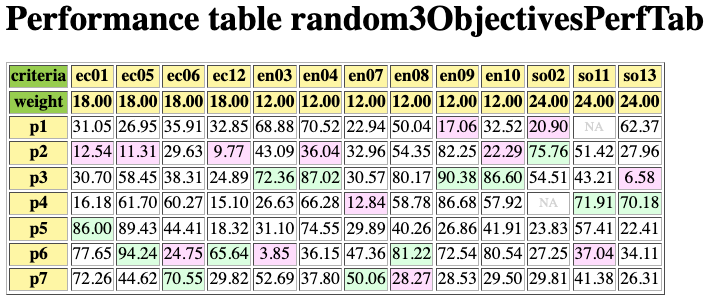
\includegraphics[width=\hsize]{Figures/6-3-random3ObjPerfTab.png}
\caption{Browser view on the given random three-objectives performance tableau.}
\label{fig:6.3}       % Give a unique label
\end{figure}

Light green cells show best performances and light red worst performances. Policy \texttt{p1} shows thus the worst performance ($17.09/100.00$) on the environmental criterion \texttt{en09}, whereas policy \texttt{p3} shows the best performances on four out of the six \emph{environmental} criteria.

No trivial best choice becomes apparent when looking at the performance tableau shown in Figure~\vref{fig:6.3}. Let us therefore compute a \Rubis best choice recommendation (see Chapter~\vref{sec:4}).
\begin{lstlisting}[caption={What is the public policy to recommend as best choice ?},label=list:6.4]
>>> from outrankingDigraphs import\
...       BipolarOutrankingDigraph
>>> g = BipolarOutrankingDigraph(t)
>>> g.showBestChoiceRecommendation()
  ***********************
  Rubis best choice recommendation(s) (BCR)
  (in decreasing order of determinateness)   
  Credibility domain: [-1.00,1.00]
  === >> potential best choice(s)
  * choice              : ['p3', 'p4', 'p5', 'p6']
   independence        : 0.00
   dominance           : 0.17
   absorbency          : -1.00
   covering (%)        : 41.67
   determinateness (%) : 52.98
   - most credible action(s) = { 'p3': 0.17, }
  === >> potential worst choice(s) 
  * choice              : ['p1', 'p2', 'p5', 'p7']
   independence        : 0.00
   dominance           : -0.44
   absorbency          : 0.19
   covered (%)         : 41.67
   determinateness (%) : 50.79
   - most credible action(s) = { 'p7': 0.06, }
\end{lstlisting}

Policy \texttt{p3} gives the most credible best choice candidate with the support of a $57.5\%$ majority of significance, whereas policy \texttt{p7} appears to be the weakest choice. Policy \texttt{p5} gives an ambiguous best and worst choice candidate. A drawing of the strict outranking digraph oriented by best and worst choices gives a more complete preferential picture (see Fig.~\vref{fig:6.4}).
\begin{lstlisting}
>>> (~(-g)).exportGraphViz(\
...             fileName='3ObjPerfTabBestChoice',\
...             bestChoice=['p3'],worstChoice=['p7'])
  *---- exporting a dot file for GraphViz tools ---------*
   Exporting to 3ObjPerfTabBestChoice.dot
   dot -Grankdir=BT -Tpng 3ObjPerfTabBestChoice.dot\
                    -o 3ObjPerfTabBestChoice.png
\end{lstlisting}
\begin{figure}[ht]
\sidecaption[t]
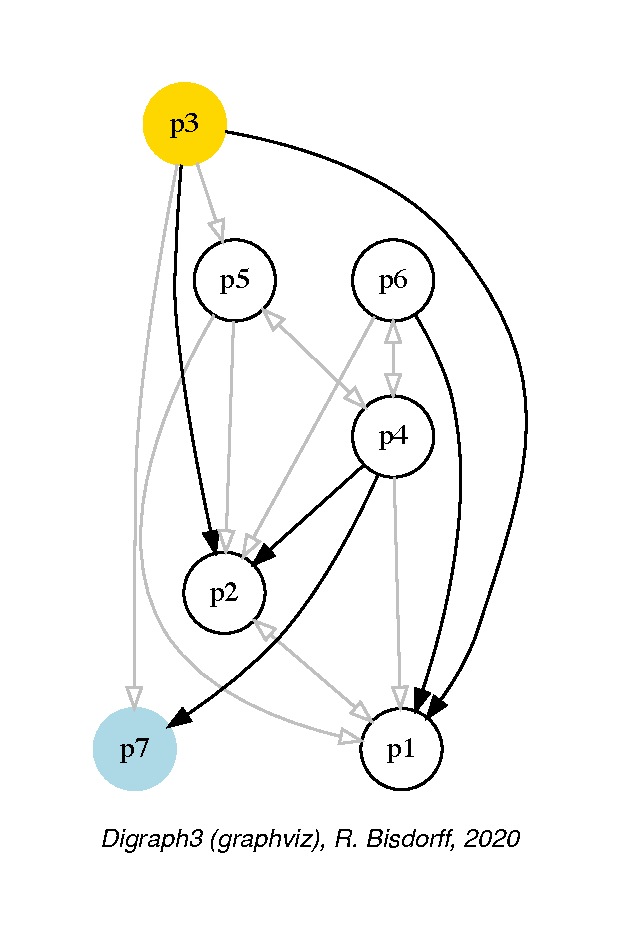
\includegraphics[width=6cm]{Figures/6-4-3ObjPerfTabBestChoice.pdf}
\caption{The strict outranking digraph oriented by best and worst choices. Policy \texttt{p5} is indeed incomparable --in a strict outranking sense-- to all the other six policies. Policies \texttt{p1}, \texttt{p2} and \texttt{p7} appear strictly outranked}
\label{fig:6.4}       % Give a unique label
\end{figure}

A heatmap view on the \Copeland ranked performance tableau confirms the best choice recommendation (see Section~\vref{sec:8.2}).
\begin{lstlisting}
>>> t.showHTMLPerformanceHeatmap(Correlations=True,\
...                        colorLevels=5,ndigits=1,\
...                        rankingRule='Copeland')
\end{lstlisting}
\begin{figure}[ht]
%\sidecaption[t]
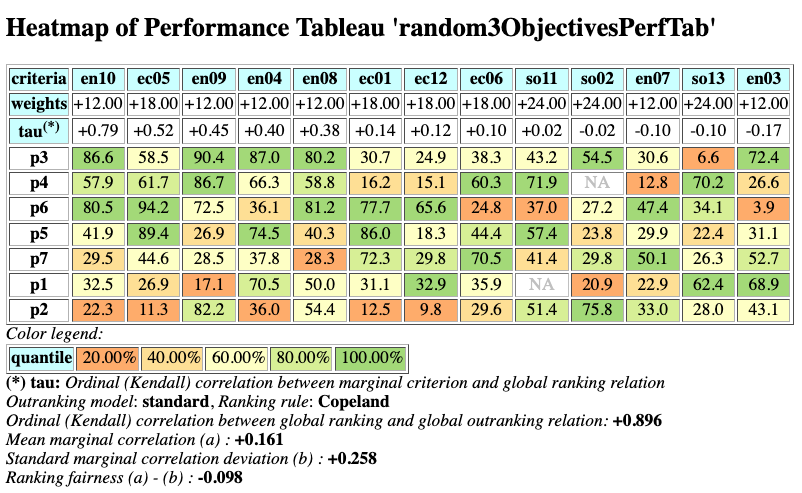
\includegraphics[width=\hsize]{Figures/random3ObjHeatmap.png}
\caption{Browser view on the \Copeland ranked performance tableau}
\label{fig:6.5}       % Give a unique label
\end{figure}

The heatmap view with its \Copeland ranking based on the bipolar outranking digraph confirms policy's \texttt{p3} as first-ranked. Notice also that the three strict outranked policies do effectively appear in the last positions. 
%\clearpage
\section{Random academic performance tableaux}
\label{sec:6.5}

The \texttt{RandomAcademicPerformanceTableau} class\index{RandomAcademicPerformanceTableau@\texttt{RandomAcademicPerformanceTableau()}} generates performance tableaux with random grades for a given number of students in different courses. 

\noindent \textbf{Generator directives:}
\begin{itemize}[leftmargin=0.5cm,rightmargin=0.5cm,topsep=1pt]
\item \texttt{numberOfStudents} := \texttt{Integer} (default 10)
\item \texttt{numberOfCourses} := \texttt{Integer} (default 5)
\item \texttt{weightDistribution} := '\emph{equisignificant}' | '\emph{random}' (default),
\item \texttt{weightScale} := $1$, $1$ - \texttt{numberOfCourses} (default when random)),
\item \texttt{IntegerWeights} := \texttt{Boolean} (True = default),
\item \texttt{commonScale} := (\texttt{Integer},\texttt{integer}) $(0,20)$ (default),
\item \texttt{ndigits} := \texttt{Integer} (default 0),
\item \texttt{WithTypes} := \texttt{Boolean} (default False),
\item \texttt{commonMode} := ('\emph{triangular}',$xm$=14,$r$=0.25) (default),
\item \texttt{commonThresholds} := {'ind':(0,0), 'pref':(1,0)} (default),
\item \texttt{missingDataProbability} := 0.0 (default),
\item \texttt{NA} := \texttt{Decimal} (default = $-999$); missing data symbol. 
\end{itemize}      

When Parameter \texttt{WithTypes} is set to \texttt{True}, the students are randomly allocated to one of the following four categories --\emph{weak} (1/6), \emph{fair} (1/3), \emph{good} (1/3), and \emph{excellent} (1/3)-- in the bracketed proportions. In a default $0-20$ grading range, the random range of a weak student is $0-10$, of a fair student $4-16$, of a good student $8-20$, and of an excellent student $12-20$. The random grading generator follows in this case a double triangular probability law with \emph{mode} ($xm$) equal to the middle of the random range and median repartition ($r = 0.5$) of probability each side of the mode.
\begin{lstlisting}[caption={Generating a random academic performance tableau},label=list:6.5]
>>> from randomPerfTabs import RandomAcademicPerformanceTableau
>>> t = RandomAcademicPerformanceTableau(\
...        numberOfStudents=11,\
...        numberOfCourses=7, missingDataProbability=0.03,\
...        WithTypes=True, seed=100)
>>> t
  *------- PerformanceTableau instance description ------*
   Instance class   : RandomAcademicPerformanceTableau
   Seed             : 100
   Instance name    : randstudPerf
   Actions          : 11
   Criteria         : 7
   NA proportion(%) : 5.2
   Attributes       : ['randomSeed', 'name', 'actions',
             'criteria', 'evaluation', 'weightPreorder']
>>> t.showPerformanceTableau()
  *----  performance tableau -----*
   Courses |   'm1'  'm2'  'm3'  'm4'  'm5'  'm6'  'm7' 
     ECTS  |    2     1     3     4     1     1     5    
  ---------|------------------------------------------
    's01f' |    12    13    15    08    16    06    15   
    's02g' |    10    15    20    11    14    15    18   
    's03g' |    14    12    19    11    15    13    11   
    's04f' |    13    15    12    13    13    10    06   
    's05e' |    12    14    13    16    15    12    16   
    's06g' |    17    13    10    14    NA    15    13   
    's07e' |    12    12    12    18    NA    13    17   
    's08f' |    14    12    09    13    13    15    12   
    's09g' |    19    14    15    13    09    13    16   
    's10g' |    10    12    14    17    12    16    09   
    's11w' |    10    10    NA    10    10    NA    08
>>> t.weightPreorder
  [['m2', 'm5', 'm6'], ['m1'], ['m3'], ['m4'], ['m7']]
\end{lstlisting}
  
The example random tableau, generated for instance above with \texttt{missingData\-Proba\-bility} = $0.03$, \texttt{WithTypes} = \texttt{True} and \texttt{seed} = 100 (see List.~\vref{list:6.5} Lines 2-5), results in a set of two excellent (\texttt{s05e} and \texttt{s07e}), five good (\texttt{s02g}, \texttt{s03g}, \texttt{s06g}, \texttt{s09g} and \texttt{s10g}), three fair (\texttt{s01f}, \texttt{s04f} and \texttt{s08f}) and one weak (\texttt{s11w}) students. Notice that six students get a grade below the course validating threshold of $10$ and we observe four missing grades (\texttt{NA}), two in course \texttt{m5} and, one in courses \texttt{m3} and \texttt{m6} (see Lines 21-31).

A statistical summary of the students' grades obtained in the highest weighted course, namely \texttt{m7}, is shown with the \texttt{showCourseStatistics()} method. \index{showCourseStatistics@\texttt{showCourseStatistics()}}
\begin{lstlisting}[caption={Student performance summary statistics per course},label=list:6.6]
>>> t.showCourseStatistics('m7')
  *----- Summary performance statistics ------*
   Course name    : m7
   Course weight  : 5
   Students       : 11
   Grading scale  : 0.00 - 20.00
   Missing evaluations : 0
   Mean evaluation       : 12.82
   Standard deviation    : 3.79
   Maximal evaluation    : 18.00
   Quantile Q3 (x_75)    : 16.25
   Median evaluation     : 14.00
   Quantile Q1 (x_25)    : 10.50
   Minimal evaluation    : 6.00
   Mean absolute difference      : 4.30
   Standard difference deviation : 5.35
\end{lstlisting}

In Listing~\vref{list:6.6}, the Course \texttt{m7} evaluation statistics show a mean grade of $12.82$ and a median grade of $14$. Maximal (resp. minimal) grade is $18$ (resp. $6$).

\begin{figure}[ht]
%\sidecaption[t]
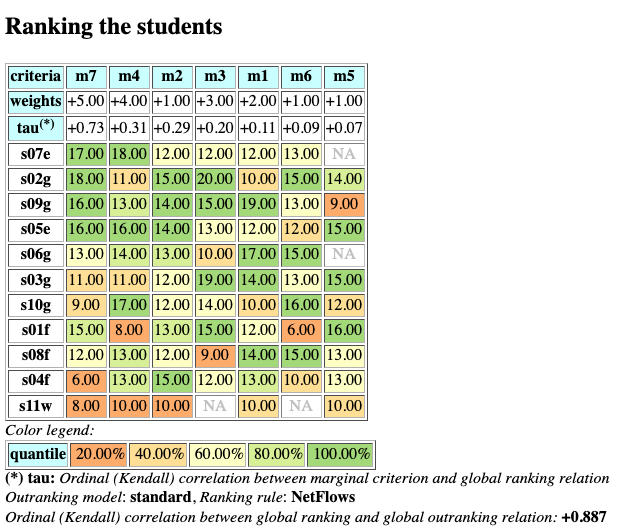
\includegraphics[width=\hsize]{Figures/6-6-rankingStudents.png}
\caption{Ranking the students in a performance heatmap view}
\label{fig:6.6}       % Give a unique label
\end{figure}
With a ranked heatmap view on all the grades we now get in Figure~\vref{fig:6.6} a global pictures of the performance of all the eleven students. The ranking shown here, produced with the \NetFlows ranking rule (see Sec.~\ref{sec:8.3}), reports a high correlation of $+0.887$ with the corresponding bipolar-valued outranking digraph (see Chapter~\ref{sec:16}).

The \NetFlows ranking represents also a rather \emph{fair weighted consensus} between the individual courses' marginal rankings as is made apparent with the \texttt{showRankingConsensusQuality()} method in Listing~\vref{list:6.7}.\index{showRankingConsensusQuality@\texttt{showRankingConsensusQuality()}}
\begin{lstlisting}[caption={Consensus quality of the students's ranking},label=list:6.7]
>>> from outrankingDigraphs import\
...                  BipolarOutrankingDigraph
>>> g = BipolarOutrankingDigraph(t)
>>> t.showRankingConsensusQuality(\
...                 g.computeNetFlowsRanking())
  Consensus quality of ranking:
  ['s07', 's02', 's09', 's05', 's06', 's03', 's10',
   's01', 's08', 's04', 's11']
  Criterion (weight): correlation
  -------------------------------
     'm7' (0.294): +0.727
     'm4' (0.235): +0.309
     'm2' (0.059): +0.291
     'm3' (0.176): +0.200
     'm1' (0.118): +0.109
     'm6' (0.059): +0.091
     'm5' (0.059): +0.073
  Summary:
   Weighted mean marginal correlation (a): +0.361
   Standard deviation (b)                : +0.248
   Ranking fairness (a)-(b)              : +0.113
\end{lstlisting}

The correlation with the marginal course rankings follows precisely the order of the given ECTS weights. Course \texttt{m7}, with the highest relative weight ($0.294$) is most present ($+0.727$) in the global \NetFlows ranking and no marginal course ranking appears negatively correlated with this global ranking. The mean weighted correlation is $+0.361$.

\vspace{1cm}
Useful multiple criteria ranking rules are presented and discussed in detail in Chapter~\ref{sec:8}. The next Chapter~\ref{sec:7} is concerned with yet another kind of performance evaluation models, namely \emph{linear voting profiles} who are discussed in social choice theory.

%%%%%%%
%The chapter bibliography
%\normallatexbib
\clearpage
%\phantomsection
%\addcontentsline{toc}{section}{Chapter Bibliography}
\bibliographystyle{spbasic}
%\typeout{}
\bibliography{03-backMatters/reference}
%\chapter{Rating by ranking with learned performance quantile norms}
\label{sec:10}

\abstract*{ We address in Chapter~\ref{sec:10} the problem of rating multiple-criteria performances of a set of potential decision alternatives with respect to performance quantiles learned from historical performance data gathered from similar decision alternatives observed in the past. We show how to learn performance quantiles from historical performance tableaux. New performance records may now be rated with respect to these quantile norms.}

\abstract{ We address in Chapter~\ref{sec:10} the problem of rating multiple-criteria performances of a set of potential decision alternatives with respect to performance quantiles learned from historical performance data gathered from similar decision alternatives observed in the past. We show how to learn performance quantiles from historical performance tableaux. New performance records may now be rated with respect to these quantile norms.}

\section{The absolute rating problem}
\label{sec:10.1}
	  
To illustrate the \emph{absolute rating} problem we face, consider for a moment that, in a given decision making problem we observe, for instance, in Table~\vref{tab:10.1} below, the multi-criteria performance evaluations of two potential decision alternatives, named \texttt{a1001} and \texttt{a1010}, evaluated on 7 \emph{incommensurable} performance criteria: 2 \emph{Costs} criteria \texttt{c1} and \texttt{c2} (to \emph{minimise}) and 5 \emph{Benefits} criteria \texttt{b1} to \texttt{b5} (to \emph{maximise}). 
\begin{table}[ht]
\caption{Multi-criteria performances of two potential decision alternatives}
\label{tab:10.1}       % Give a unique label
\begin{center}
  %\begin{small}
    \begin{tabular}{l|c|c|c|c|c|c|c}
      \svhline\noalign{\smallskip}
      Criterion (weight) & \texttt{b1} (2) & \texttt{b2} (2) & \texttt{b3} (2) & \texttt{b4} (2) & \texttt{b5} (2) & \texttt{c1} (5) & \texttt{c2} (5)\\
      \noalign{\smallskip}\hline\noalign{\smallskip}
    \texttt{a1001} &   37.0  &  2 & 2 & 61.0 & 31.0 & -4 & -40.0\\
    \texttt{a1010} &   32.0 & 9 & 6 & 55.0 & 51.0 & -4 & -35.0 \\
      \noalign{\smallskip}\hline
    \end{tabular}
  %\end{small}
\end{center}
\end{table}

The performance on \emph{Benefits} criteria \texttt{b1}, \texttt{b4} and \texttt{b5} is measured on a cardinal scale from $0.0$ (worst) to $100.0$ (best) whereas, the performance on the \emph{Benefits} criteria \texttt{b2} and \texttt{b3}  and on the \emph{Costs} criterion \texttt{c1} is measured on an ordinal scale from $0$ (worst) to $10$ (best), respectively $-10$ (worst) to $0$ (best). The performance on the \emph{Costs} criterion \texttt{c2} is eventually measured on a cardinal \emph{negative} scale from $-100.00$ (worst) to $0.0$ (best). The two \emph{Costs} criteria are equi-significant (weight 5). Similarly, the five Benefits criteria are also equi-significant (weight 2). The \emph{importance} (sum of significance weights: $2 \times 5 = 10$) of the \emph{Costs} criteria is hence \emph{equivalent} to the \emph{importance} (sum of significance weights: $5 \times 2 = 10$) of the \emph{Benefits} criteria.
   
The non trivial decision problem we now face, is to decide, how the previous two multiple-criteria performance records of alternatives \texttt{a1001}, respectively \texttt{a1010},  may be rated: \emph{excellent}~? \emph{good}~?, or \emph{fair}~?; perhaps even, \emph{weak}~? or \emph{very weak}~? when compared with similar multi-criteria performance records one has already rated into quantiles in the past. 

To solve this \emph{absolute} rating problem, first, we need to estimate multi-criteria \emph{performance quantiles} from historical records \citep{CPSTAT-L5}.  

\section{Incremental learning of historical performance quantiles}
\label{sec:10.2}

Suppose that we see flying in random multiple-criteria performances from a given model of random performance tableau (see Chap.~\ref{sec:5}). The question we address here is to estimate empirical performance quantiles on the basis of so far observed performance vectors. For this task, we are inspired by \citet*{CHAM-2006}, who present an efficient algorithm for incrementally updating a quantile-binned cumulative distribution function (CDF) with newly observed CDFs\footnote{We have adapted in Python a C++ implementation published by \citep*[Chapter 5]{NR3-2007}.}. 

The \texttt{PerformanceQuantiles}\index{PerformanceQuantiles@\texttt{PerformanceQuantiles} class} class, using the \texttt{IncrementalQuan\-tiles\-Estimator} class\index{IncrementalQuantilesEstimator@\texttt{IncrementalQuantilesEstimator} class} from the \texttt{randomNumbers} module \index{randomNumbers@\texttt{randomNumbers} module}, implements such a performance quantiles estimation based on a given performance tableau \citep{BIS-2021b}.

Its main attributes are:
\begin{itemize}[rightmargin=0.5cm,leftmargin=0.5cm,topsep=1pt]
\item Ordered \texttt{objectives} and a \texttt{criteria} dictionaries from a valid performance tableau instance;
\item A list \texttt{quantileFrequencies} of quantile frequencies like:
  \begin{itemize}[nosep]
  \item \emph{quartiles} $[0.0, 0.25, 05, 0.75,1.0]$,
  \item  \emph{quintiles} $[0.0, 0.2, 0.4, 0.6, 0.8, 1.0]$ or
  \item  \emph{deciles} $[0.0, 0.1, 0.2, ... 1.0]$ for instance;
  \end{itemize}
\item An ordered  dictionary \texttt{limitingQuantiles} of so far estimated \emph{lower} (default) or \emph{upper} quantile class limits for each frequency per criterion;
\item An ordered dictionary \texttt{historySizes} for keeping track of the number of evaluations seen so far per criterion. Missing data, the case given, make these sizes vary from criterion to criterion.
\end{itemize}

Below, we show an example Python session concerning 900 decision alternatives randomly generated with a \emph{Cost-Benefit} performance tableau model (see Sec.~\ref{sec:5.3}) from which are also drawn the performances of alternatives \texttt{a1001} and \texttt{a1010} shown in Table~\vref{tab:10.1} above.
\begin{lstlisting}[caption={Computing performance quantiles from a given performance tableau},label=list:10.1]
>>> from performanceQuantiles import PerformanceQuantiles
>>> from randomPerfTabs import RandomCBPerformanceTableau
>>> nbrActions=900
>>> nbrCrit = 7
>>> seed = 100
>>> pt = RandomCBPerformanceTableau(numberOfActions=nbrActions,\
...                  numberOfCriteria=nbrCrit,seed=seed)
>>> pq = PerformanceQuantiles(pt,\
...                   numberOfBins = 'quartiles',\
...                   LowerClosed=True)
>>> pq
  *------- PerformanceQuantiles instance description ------*
   Instance class   : PerformanceQuantiles
   Instance name    : 4-tiled_performances
   Objectives       : 2
   Criteria         : 7
   Quantiles        : 4
   History sizes    : {'c1': 887,'b1': 888,'b2': 891,'b3': 895,
                        'b4': 892,'c2': 893,'b5': 887}
   Attributes       : ['perfTabType','valueDigits',
                       'actionsTypeStatistics',
                       'objectives', 'BigData',
                       'missingDataProbability',
		       'criteria', 'LowerClosed', 'name',
		       'quantilesFrequencies', 'historySizes',
		       'limitingQuantiles', 'cdf']
\end{lstlisting}
The \texttt{PerformanceQuantiles} class parameter \texttt{numberOfBins} (see List.~\vref{list:10.1} Line 9 above), choosing the wished number of quantile frequencies, may be either \emph{quartiles} (4 bins), \emph{quintiles} (5 bins), \emph{deciles} (10 bins), \emph{dodeciles} (20 bins) or any other integer number of quantile bins. The quantile bins may be either \emph{lower closed} (default) or \emph{upper-closed}.

Inspecting the estimated quartile limits may be operated with the\\ \texttt{showLimitingQuantiles()} method.\index{showLimitingQuantiles@\texttt{showLimitingQuantiles()}}
\begin{lstlisting}[caption={Printing out the estimated quartile limits},label=list:10.2]
>>> pq.showLimitingQuantiles(ByObjectives=True)
    ----  Historical performance quantiles -----*
    Costs
    criteria | weights |  '0.00' '0.25' '0.50' '0.75' '1.00'   
    ---------|----------------------------------------------------
       'c1'  |    5    |   -10    -7     -5     -3      0  
       'c2'  |    5    | -96.37 -70.65 -50.10 -30.00  -1.43  
    Benefits
    criteria | weights | '0.00'  '0.25' '0.50' '0.75' '1.00'   
    ---------|-----------------------------------------------------
       'b1'  |    2    |  1.99    29.82 49.44  70.73  99.83  
       'b2'  |    2    |    0      3      5      7     10  
       'b3'  |    2    |    0      3      5      7     10  
       'b4'  |    2    |  3.27   30.10  50.82  70.89  98.05  
       'b5'  |    2    |  0.85   29.08  48.55  69.98  97.56  
\end{lstlisting}
Both objectives are \emph{equally important}; the sum of weights (10) of the \emph{Costs} criteria balance the sum of weights (10) of the \emph{Benefits} criteria (see List.~\vref{list:10.2} column 2). The preference direction of the \emph{Costs} criteria \texttt{c1} and \texttt{c2} is \emph{negative}; the lesser the costs, the better it is, whereas all the \emph{Benefits} criteria \texttt{b1} to \texttt{b5} show \emph{positive} preference directions, i.e. the higher the benefits, the better it is. The columns entitled '$0.00$', resp. '$1.00$' show the \emph{quartile} \texttt{Q0}, resp. \texttt{Q4}, i.e. the \emph{worst}, resp. \emph{best} performance observed so far on each criterion. Column '$0.50$' shows the \emph{median} (\texttt{Q2}) performance observed on the criteria.  

New  decision alternatives with random multiple-criteria performance vectors from the same random performance tableau model as \texttt{pt} (see List.~\vref{list:10.1}) may now be generated with a generic \texttt{RandomPerformanceGenerator} class\index{RandomPerformanceGenerator@\texttt{RandomPerformanceGenerator()}} from the \texttt{randomPerfTabs} module \citep{BIS-2021b}.\footnote{The \texttt{RandomPerformanceGenerator} class works for the \emph{standard} performance tableau model (see Sec.~\ref{sec:5.2}), the \emph{Cost-Benefit} model (see Sec.~\ref{sec:5.3}), and the 3-objectives model (see Sec.~\ref{sec:5.4}).}
\begin{lstlisting}[caption={Generating 100 new random decision alternatives of the same model},label=list:10.3]
>>> from randomPerfTabs import RandomPerformanceGenerator
>>> rpg = RandomPerformanceGenerator(tp,seed=seed)
>>> newTab = rpg.randomPerformanceTableau(100)
\end{lstlisting}

The so far estimated historical quantile limits must, first, be updated with this newly arriving 100 data records:
\begin{lstlisting}
>>> # Updating the quartile norms shown above 
>>> pq.updateQuantiles(newTab,historySize=None)
\end{lstlisting}
Parameter \texttt{historySize} of the \texttt{updateQuantiles()} method\index{updateQuantiles@\texttt{updateQuantiles()}} (Line 2 above) allows to \emph{balance} the \emph{new} evaluations against the \emph{historical} ones.

With \texttt{historySize = None} (the default setting), the balance in the example above is $900/1000$ ($90\%$, the weight of historical data) against $100/1000$ ($10\%$, the weight of the new incoming observations). Setting \texttt{historySize = 0}, for instance, will ignore all historical data ($0/100$ against $100/100$) and restart building the quantile estimation with solely the new incoming data. The \texttt{showHTMLLimitingQuantiles()} method\index{showHTMLLimitingQuantiles@\texttt{showHTMLLimitingQuantiles()}} shows the updated quantile limits in a browser view (see Fig.~\vref{fig:10.1}).
\begin{lstlisting}
>>> # showing the updated quantile limits in a browser view
>>> pq.showHTMLLimitingQuantiles(Transposed=True)
\end{lstlisting}
\begin{figure}[ht]
\sidecaption[t]
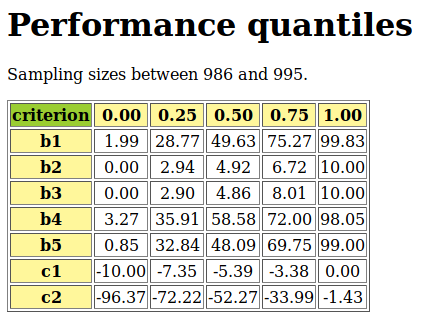
\includegraphics[width=7cm]{Figures/10-1-examplePerfQuantiles.png}
\caption[Showing updated quartiles limits per criterion]{\emph{Showing updated quartiles limits per criterion}. The $0.25$ column shows the first quartile (\texttt{Q1}) limits, the $0.50$ column shows the second quartile (\texttt{Q2}) limits and the $0.75$ column shows the third quartile (\texttt{Q3}) limits. Column $0.00$ (resp. $1.00$) shows the minimum (resp. maximum) performance on each criterion}
\label{fig:10.1}       % Give a unique label
\end{figure}
    
\section{Rating-by-ranking new performances with quantile norms}
\label{sec:10.3}

For \emph{rating} a newly given set of decision alternatives with the help of empirical performance quantiles estimated from historical data, the \texttt{sortingDigraphs} module provides the \texttt{Learned\-QuantilesRatingDigraph} class\index{LearnedQuantilesRatingDigraph@\texttt{LearnedQuantilesRatingDigraph} class}, a specialisation of the \texttt{QuantilesSor\-tingDigraph} class (see Chap.~\ref{sec:9}). The absolute rating result is computed by \emph{ranking} the new performance records together with the learned historical quantile limits.

The class constructor requires a valid \texttt{PerformanceQuantiles} instance and, by default, uses the \Copeland or the \NetFlows ranking rule, whichever fits best in an ordinal correlation sense with the underlying outranking digraph.

It is important to notice that the \texttt{LearnedQuantilesRatingDigraph} class, contrary to the generic \texttt{OutrankingDigraph} class, does not inherit from the generic \texttt{PerformanceTableau} class, but instead from the \texttt{Performance\-Quantiles} class \citep{BIS-2021b}.

The \texttt{actions} attribute in such a \texttt{LearnedQuantilesRatingDigraph} class instance contains not only the newly given decision alternatives, but also the historical quantile limits (attribute \texttt{profiles}) obtained from a given \texttt{Perfor\-manceQuantiles} class instance, i.e. estimated quantile bins' performance limits from historical performance data.

We reconsider now the \texttt{PerformanceQuantiles} object instance \texttt{pq} as computed in the previous section. Let \texttt{newActions} be a list of 10 new decision alternatives generated with the same random performance tableau generator \texttt{rpq} and including, for our didactical purpose, the two decision alternatives \texttt{a1001} and \texttt{a1010} mentioned at the beginning.
\begin{lstlisting}[caption={Computing the absolute rating of 10 new decision alternatives},label=list:10.4]
>>> from sortingDigraphs import LearnedQuantilesRatingDigraph
>>> newActions = rpg.randomActions(10)
>>> lqr = LearnedQuantilesRatingDigraph(pq,newActions,\
...                                     rankingRule='best')
>>> lqr
  *---- Object instance description
   Instance class      : LearnedQuantilesRatingDigraph
   Instance name       : normedRatingDigraph
   Criteria            : 7
   Quantile profiles   : 4
   Lower-closed bins   : True
   New actions         : 10
   Size                : 93
   Determinateness (%) : 76.1
   Ranking rule        : Copeland
   Ordinal correlation : +0.95
   Attributes: ['runTimes','objectives','criteria',
     'LowerClosed','quantilesFrequencies',
     'limitingQuantiles','historySizes','cdf','name',
     'newActions','evaluation','categories',
     'criteriaCategoryLimits','profiles','profileLimits',
     'hasNoVeto','actions','completeRelation','relation',
     'concordanceRelation','valuationdomain','order',
     'gamma','notGamma','rankingRule','rankingCorrelation',
     'rankingScores','actionsRanking','ratingCategories',
     'ratingRelation','relationOrig']
  *---- Constructor run times (in sec.)
   Threads           : 1
   Total time       : 0.02218
   Data input       : 0.00134
   Quantile classes : 0.00008
   Compute profiles : 0.00021
   Compute relation : 0.01869
   Compute rating   : 0.00186
   Compute sorting  : 0.00000
\end{lstlisting}

Data input to the \texttt{LearnedQuantilesRatingDigraph} class constructor are a valid \texttt{PerformanceQuantiles} object \texttt{pq} and a \texttt{newActions} list of newly generated decision alternatives with the same random generator \texttt{rpg} (see List.~\vref{list:10.4} Line 2-3).

The \texttt{actionsSubset} parameter of the \texttt{showPerformanceTableau()} method\index{showPerformanceTableau@\texttt{showPerformanceTableau()}} allows a look at the digraph's nodes, here called \texttt{newActions}.
\begin{lstlisting}[caption={Performance tableau of the new incoming decision alternatives},label=list:10.5,basicstyle=\ttfamily\scriptsize]
>>> lqr.showPerformanceTableau(actionsSubset=lqr.newActions)
 *----  performance tableau -----*
 criteria | a1001 a1002 a1003 a1004 a1005 a1006 a1007 a1008 a1009 a1010   
 ---------|-------------------------------------------------------------
    'b1'  |  37.0  27.0  24.0  16.0  42.0  33.0  39.0  64.0  42.0  32.0  
    'b2'  |   2.0   5.0   8.0   3.0   3.0   3.0   6.0   5.0   4.0   9.0  
    'b3'  |   2.0   4.0   2.0   1.0   6.0   3.0   2.0   6.0   6.0   6.0  
    'b4'  |  61.0  54.0  74.0  25.0  28.0  20.0  20.0  49.0  44.0  55.0  
    'b5'  |  31.0  63.0  61.0  48.0  30.0  39.0  16.0  96.0  57.0  51.0  
    'c1'  |  -4.0  -6.0  -8.0  -5.0  -1.0  -5.0  -1.0  -6.0  -6.0  -4.0  
    'c2'  | -40.0 -23.0 -37.0 -37.0 -24.0 -27.0 -73.0 -43.0 -94.0 -35.0  
\end{lstlisting}

Among the 10 new incoming decision alternatives, we recognise alternatives \texttt{a1001} (see column 2) and \texttt{a1010} (see last column) we have shown in Table~\vref{tab:10.1}.

The \texttt{actions} dictionary of a \texttt{LearnedQuantilesRatingDigraph} class instance includes, besides the 10 performance evaluations of the ten new alternatives, also the closed lower limits of the four quartile classes: \texttt{m1} = $[0.0- [$, \texttt{m2} = $[0.25- [$, \texttt{m3} = $[0.5- [$, \texttt{m4} = $[0.75 - [$. We find these limits in the \texttt{profiles} attribute (see List.~\vref{list:10.6} below).
\begin{lstlisting}[caption={Showing the limiting profiles of the rating quantiles},label=list:10.6]
>>> lqr.showPerformanceTableau(actionsSubset=lqr.profiles)
    *----  Quartiles limit profiles -----*
    criteria |  'm1'   'm2'   'm3'   'm4'   
    ---------|----------------------------
       'b1'  |  2.0    28.8   49.6   75.3  
       'b2'  |  0.0     2.9    4.9    6.7  
       'b3'  |  0.0     2.9    4.9    8.0  
       'b4'  |  3.3    35.9   58.6   72.0  
       'b5'  |  0.8    32.8   48.1   69.7  
       'c1'  | -10.0   -7.4   -5.4   -3.4  
       'c2'  | -96.4  -72.2  -52.3  -34.0  
\end{lstlisting}

The main run time is spent by the \texttt{LearnedQuantilesRatingDigraph} class constructor in computing a bipolar-valued outranking relation on the extended actions set including both the new alternatives as well as the quartile class limits (see List.~\vref{list:10.4} Lines 23-29).\footnote{In case of large volumes, i.e. many new decision alternatives and centile classes for instance, a multi-threading version may be used when multiple processing cores are available \citep{BIS-2021b}.}

The actual rating procedure will rely on a complete ranking of the new decision alternatives as well as the quantile class limits obtained from the corresponding bipolar-valued outranking digraph. Two efficient and scalable ranking rules, the \Copeland and its valued version, the \NetFlows rule may be used for this purpose. The \texttt{rankingRule} parameter allows to choose one of both. With \texttt{rankingRule='best'} (see List.~\vref{list:10.4} Line 3 ) the \texttt{LearnedQuantiles\-RatingDigraph} constructor will choose the ranking rule that results in the highest ordinal correlation with the given outranking relation (see Chap.~\ref{sec:22} and \citep{BIS-2012a}).

In this rating example, the \Copeland rule appears to be the more appropriate ranking rule.
\begin{lstlisting}[caption={\Copeland ranking of new alternatives and historical quartile limits},label=list:10.7]
>>> lqr.rankingRule
  'Copeland'
>>> lqr.actionsRanking
  ['m4', 'a1005', 'a1010', 'a1002', 'a1008', 'a1006', 'a1001',
   'a1003', 'm3', 'a1007', 'a1004', 'a1009', 'm2', 'm1'] 
>>> lqr.showCorrelation(lqr.rankingCorrelation)
  Correlation indexes:
    Crisp ordinal correlation  : +0.945
    Epistemic determination    :  0.522
    Bipolar-valued equivalence : +0.493
\end{lstlisting}

We achieve here in Listing.~\vref{list:10.7} a linear ranking without ties (from best to worst) of the digraph's actions set, i.e. including the new decision alternatives as well as the quartile limits $m1$ to $m4$, which is very close in an ordinal sense ($\tau = 0.945$) to the underlying strict outranking relation.

The eventual rating procedure is based in this example on the \emph{lower} quartile limits, such that the quartile classes' contents are filtered out in increasing order of the \emph{quartiles}.
\begin{lstlisting}
>>> lqr.ratingCategories
 OrderedDict([
 ('m2', ['a1007','a1004','a1009']),
 ('m3', ['a1005','a1010','a1002','a1008',
         'a1006','a1001','a1003'])
 ])
\end{lstlisting}    

We notice above that no new decision alternative is actually rated into the lowest $[0.0-0.25[$, respectively highest $[0.75- [$ quartile classes. Indeed, the absolute rating result is shown with the \texttt{showQuantilesRating()} method\index{showQuantilesRating@\texttt{showQuantilesRating()}}:
\begin{lstlisting}[caption={Absolute quartiles rating result},label=list:10.8]
>>> lqr.showQuantilesRating()
  *-------- Quartiles rating result ---------
   [0.50 - 0.75[ ['a1005', 'a1010', 'a1002', 'a1008',
                  'a1006', 'a1001', 'a1003']
   [0.25 - 0.50[ ['a1007', 'a1004', 'a1009']
\end{lstlisting}    

The same result may also be shown in a browser view with the \texttt{showHTMLRa\-tingHeatmap()} method\index{showHTMLRatingHeatmap@\texttt{showHTMLRatingHeatmap()}} using a specialised rating heatmap format (see Fig.~\vref{fig:10.2}): 
\begin{lstlisting}
>>> lqr.showHTMLRatingHeatmap(\
...            pageTitle='Heatmap of Quartiles Rating',\
...            Correlations=True,colorLevels=5)
\end{lstlisting}
\begin{figure}[ht]
\sidecaption[t]
 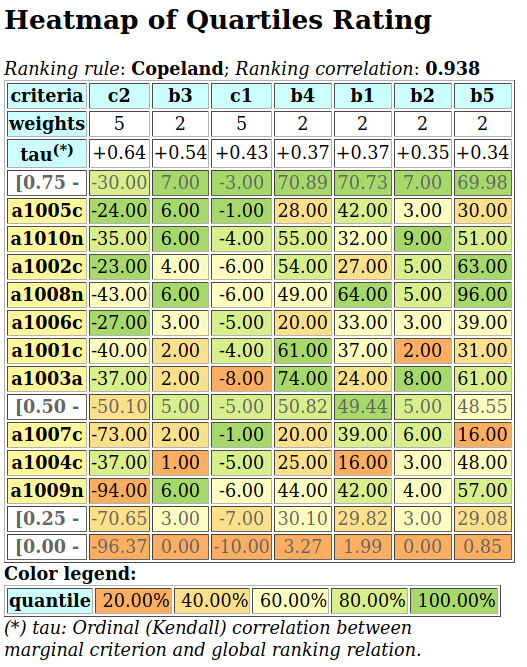
\includegraphics[width=7cm]{Figures/10-2-heatMap1.png}
\caption[Heatmap of absolute quartiles ranking]{\emph{Heatmap of absolute quartiles ranking}. The quartile equivalence classes appear lower-closed. No alternative is rated into the \texttt{Q1} class ($[0.00 - 0.25[$) and no alternative is rated into the Q4 class ($[0.75 - 1.00]$)}
\label{fig:10.2}       % Give a unique label
\end{figure}
	    
Using furthermore a specialised version of the \texttt{exportGraphViz()} method allows drawing in Figure~\vref{fig:10.3} the same rating result in a Hasse diagram format.\footnote{Note that the graphviz dot file was post-edited in order to mark in blue alternatives \texttt{a1001} and \texttt{a1010}.}
\begin{lstlisting}
>>> lqr.exportRatingGraphViz('quartileRatingDigraph')
 *---- exporting a dot file for GraphViz tools ---------*
  Exporting to quartileRatingDigraph.dot
  dot -Grankdir=TB -Tpng quartileRatingDigraph.dot -o quartileRatingDigraph.png
\end{lstlisting}
\begin{figure}[ht]
%\sidecaption[t]
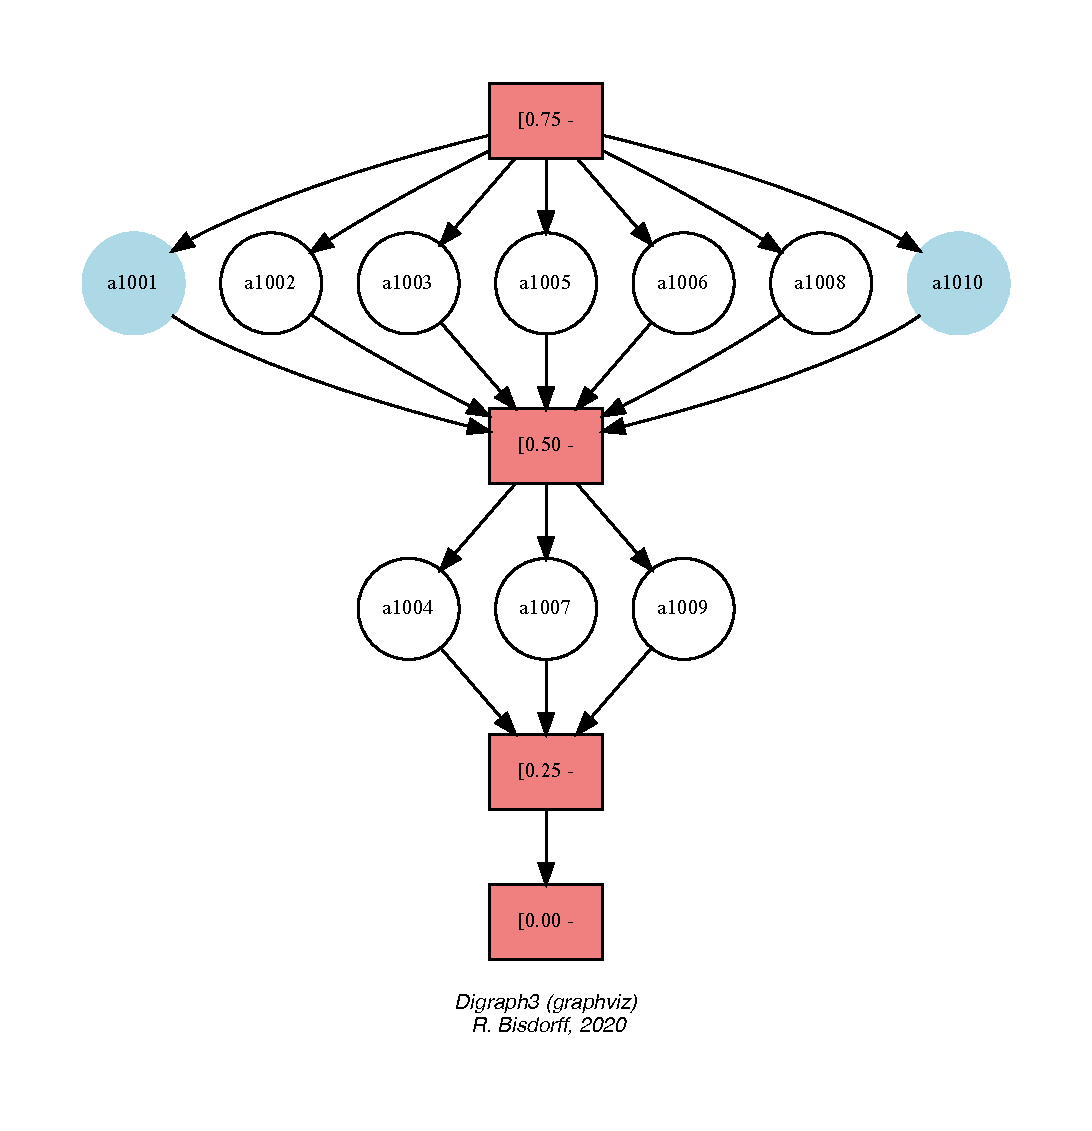
\includegraphics[width=\hsize]{Figures/10-3-normedRatingDigraph.pdf}
\caption{Absolute quartiles rating digraph}
\label{fig:10.3}       % Give a unique label
\end{figure}

We have actually solved now the \emph{absolute rating} problem stated at the beginning. Decision alternatives \texttt{a1001} and \texttt{a1010} (see Tab.~\vref{tab:10.1}) are both rated into the same third quartile \texttt{Q3} class (see Fig.~\vref{fig:10.3}), even if the \Copeland ranking, obtained from the underlying strict outranking digraph (see Fig.~\vref{fig:10.2}), suggests that alternative \texttt{a1010} is effectively \emph{better performing than} alternative \texttt{a1001}. 

A \emph{preciser} rating result may indeed be achieved when using \emph{deciles} instead of \emph{quartiles} for estimating the historical marginal cumulative distribution functions.
\begin{lstlisting}[caption={Absolute deciles rating result},label=list:10.9]
>>> pq1 = PerformanceQuantiles(pt, numberOfBins = 'deciles',\
...                 LowerClosed=True)
>>> pq1.updateQuantiles(newTab,historySize=None)
>>> lqr1 = LearnedQuantilesRatingDigraph(pq1,newActions,rankingRule='best')
>>> lqr1.showQuantilesRating()
  *-------- Deciles rating result ---------
   [0.60 - 0.70[ ['a1005', 'a1010', 'a1008', 'a1002']
   [0.50 - 0.60[ ['a1006', 'a1001', 'a1003']
   [0.40 - 0.50[ ['a1007', 'a1004']
   [0.30 - 0.40[ ['a1009']
\end{lstlisting}

Compared with the quartiles rating result, we notice in Listing~\vref{list:10.9} that the seven alternatives (\texttt{a1001}, \texttt{a1002}, \texttt{a1003}, \texttt{a1005}, \texttt{a1006}, \texttt{a1008} and \texttt{a1010}), rated before into the third quartile class $[0.50-0.75[$, are now divided up: alternatives \texttt{a1002}, \texttt{a1005}, \texttt{a1008} and \texttt{a1010} attain now the 7th decile class $[0.60-0.70[$, whereas alternatives \texttt{a1001}, \texttt{a1003} and \texttt{a1006} attain only the 6th decile class $[0.50-0.60[$. Of the three \texttt{Q2} $[0.25-0.50[$ rated alternatives (\texttt{a1004}, \texttt{a1007} and \texttt{a1009}), alternatives \texttt{a1004} and \texttt{a1007} are now rated into the 5th decile class $[0.40-0.50[$ and \texttt{a1009} is lowest rated into the 4th decile class $[0.30-0.40[$.

A browser heatmap view in Figure~\vref{fig:10.4} more conveniently illustrates this refined rating result.
\begin{lstlisting}
>>> lqr1.showHTMLRatingHeatmap(\
...       pageTitle='Heatmap of the deciles rating',\
...       colorLevels=5, Correlations=True)
\end{lstlisting}
\begin{figure}[ht]
\sidecaption[t]
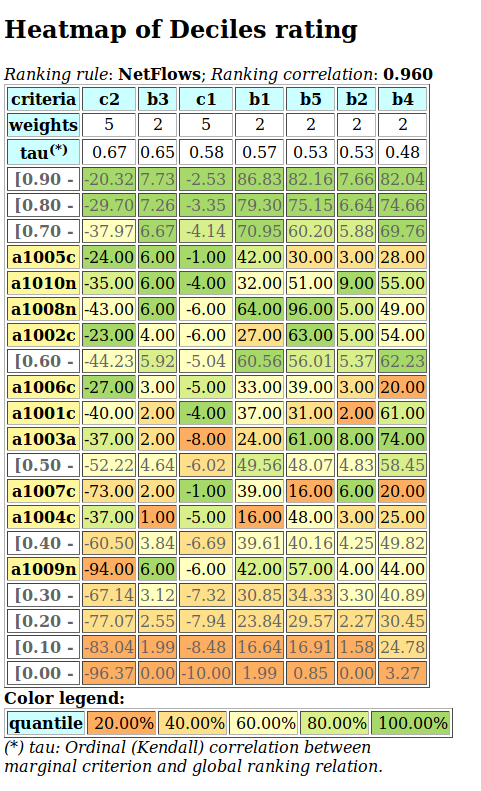
\includegraphics[width=7cm]{Figures/10-4-heatMap2.png}
\caption[Heatmap of absolute deciles rating]{\emph{Heatmap of absolute deciles rating}. Decision alternatives \texttt{a1001} and \texttt{a1010} are now, as expected, rated in the $6^{th}$ decile (\texttt{D6}), respectively in the $7^{th}$ decile (\texttt{D7})}
\label{fig:10.4}       % Give a unique label
\end{figure}

To avoid having to recompute performance deciles from historical data when wishing to refine a rating result, it is useful, depending on the actual size of the historical data, to initially compute performance quantiles with a relatively high number of bins, for instance \emph{dodeciles} or even \emph{centiles}. It is then possible to interpolate on the fly \emph{quartiles} or \emph{deciles} for instance, when constructing the rating digraph. 
\begin{lstlisting}[caption={From deciles interpolated quartiles rating result},label=list:10.10]
>>> lqr2 = LearnedQuantilesRatingDigraph(pq1,newActions,
...                   quantiles='quartiles')
>>> lqr2.showQuantilesRating()
  *-------- Deciles rating result ---------
   [0.50 - 0.75[ ['a1005', 'a1010', 'a1002', 'a1008',
                  'a1006', 'a1001', 'a1003']
   [0.25 - 0.50[ ['a1004', 'a1007', 'a1009']
\end{lstlisting}

With the \texttt{quantiles} parameter (see List.~\vref{list:10.10} Line 2), we recover by interpolation the same quartiles rating as obtained directly with historical performance quartiles (see List.~\vref{list:10.8}). Mind that a correct interpolation of quantiles from a given cumulative distribution function requires more or less uniform distributions of observations in each bin. 
More generally, in the case of industrial production monitoring problems, for instance, where large volumes of historical performance data may be available, it can be of interest to estimate even more precisely the marginal cumulative distribution functions, especially when \emph{tail} rating results, i.e. distinguishing \emph{very best}, or \emph{very weak} multiple-criteria performances, become a critical issue. Similarly, the \texttt{historySize} parameter may be used for monitoring on the fly \emph{unstable} random multiple-criteria performance data \citep{CHAM-2006}.  	

%%%%%%%
%The chapter bibliography
%\normallatexbib
%\clearpage
%\phantomsection
%\addcontentsline{toc}{section}{References}
%\chapter{Rating by ranking with learned performance quantile norms}
\label{sec:10}

\abstract*{ We address in Chapter~\ref{sec:10} the problem of rating multiple-criteria performances of a set of potential decision alternatives with respect to performance quantiles learned from historical performance data gathered from similar decision alternatives observed in the past. We show how to learn performance quantiles from historical performance tableaux. New performance records may now be rated with respect to these quantile norms.}

\abstract{ We address in Chapter~\ref{sec:10} the problem of rating multiple-criteria performances of a set of potential decision alternatives with respect to performance quantiles learned from historical performance data gathered from similar decision alternatives observed in the past. We show how to learn performance quantiles from historical performance tableaux. New performance records may now be rated with respect to these quantile norms.}

\section{The absolute rating problem}
\label{sec:10.1}
	  
To illustrate the \emph{absolute rating} problem we face, consider for a moment that, in a given decision making problem we observe, for instance, in Table~\vref{tab:10.1} below, the multi-criteria performance evaluations of two potential decision alternatives, named \texttt{a1001} and \texttt{a1010}, evaluated on 7 \emph{incommensurable} performance criteria: 2 \emph{Costs} criteria \texttt{c1} and \texttt{c2} (to \emph{minimise}) and 5 \emph{Benefits} criteria \texttt{b1} to \texttt{b5} (to \emph{maximise}). 
\begin{table}[ht]
\caption{Multi-criteria performances of two potential decision alternatives}
\label{tab:10.1}       % Give a unique label
\begin{center}
  %\begin{small}
    \begin{tabular}{l|c|c|c|c|c|c|c}
      \svhline\noalign{\smallskip}
      Criterion (weight) & \texttt{b1} (2) & \texttt{b2} (2) & \texttt{b3} (2) & \texttt{b4} (2) & \texttt{b5} (2) & \texttt{c1} (5) & \texttt{c2} (5)\\
      \noalign{\smallskip}\hline\noalign{\smallskip}
    \texttt{a1001} &   37.0  &  2 & 2 & 61.0 & 31.0 & -4 & -40.0\\
    \texttt{a1010} &   32.0 & 9 & 6 & 55.0 & 51.0 & -4 & -35.0 \\
      \noalign{\smallskip}\hline
    \end{tabular}
  %\end{small}
\end{center}
\end{table}

The performance on \emph{Benefits} criteria \texttt{b1}, \texttt{b4} and \texttt{b5} is measured on a cardinal scale from $0.0$ (worst) to $100.0$ (best) whereas, the performance on the \emph{Benefits} criteria \texttt{b2} and \texttt{b3}  and on the \emph{Costs} criterion \texttt{c1} is measured on an ordinal scale from $0$ (worst) to $10$ (best), respectively $-10$ (worst) to $0$ (best). The performance on the \emph{Costs} criterion \texttt{c2} is eventually measured on a cardinal \emph{negative} scale from $-100.00$ (worst) to $0.0$ (best). The two \emph{Costs} criteria are equi-significant (weight 5). Similarly, the five Benefits criteria are also equi-significant (weight 2). The \emph{importance} (sum of significance weights: $2 \times 5 = 10$) of the \emph{Costs} criteria is hence \emph{equivalent} to the \emph{importance} (sum of significance weights: $5 \times 2 = 10$) of the \emph{Benefits} criteria.
   
The non trivial decision problem we now face, is to decide, how the previous two multiple-criteria performance records of alternatives \texttt{a1001}, respectively \texttt{a1010},  may be rated: \emph{excellent}~? \emph{good}~?, or \emph{fair}~?; perhaps even, \emph{weak}~? or \emph{very weak}~? when compared with similar multi-criteria performance records one has already rated into quantiles in the past. 

To solve this \emph{absolute} rating problem, first, we need to estimate multi-criteria \emph{performance quantiles} from historical records \citep{CPSTAT-L5}.  

\section{Incremental learning of historical performance quantiles}
\label{sec:10.2}

Suppose that we see flying in random multiple-criteria performances from a given model of random performance tableau (see Chap.~\ref{sec:5}). The question we address here is to estimate empirical performance quantiles on the basis of so far observed performance vectors. For this task, we are inspired by \citet*{CHAM-2006}, who present an efficient algorithm for incrementally updating a quantile-binned cumulative distribution function (CDF) with newly observed CDFs\footnote{We have adapted in Python a C++ implementation published by \citep*[Chapter 5]{NR3-2007}.}. 

The \texttt{PerformanceQuantiles}\index{PerformanceQuantiles@\texttt{PerformanceQuantiles} class} class, using the \texttt{IncrementalQuan\-tiles\-Estimator} class\index{IncrementalQuantilesEstimator@\texttt{IncrementalQuantilesEstimator} class} from the \texttt{randomNumbers} module \index{randomNumbers@\texttt{randomNumbers} module}, implements such a performance quantiles estimation based on a given performance tableau \citep{BIS-2021b}.

Its main attributes are:
\begin{itemize}[rightmargin=0.5cm,leftmargin=0.5cm,topsep=1pt]
\item Ordered \texttt{objectives} and a \texttt{criteria} dictionaries from a valid performance tableau instance;
\item A list \texttt{quantileFrequencies} of quantile frequencies like:
  \begin{itemize}[nosep]
  \item \emph{quartiles} $[0.0, 0.25, 05, 0.75,1.0]$,
  \item  \emph{quintiles} $[0.0, 0.2, 0.4, 0.6, 0.8, 1.0]$ or
  \item  \emph{deciles} $[0.0, 0.1, 0.2, ... 1.0]$ for instance;
  \end{itemize}
\item An ordered  dictionary \texttt{limitingQuantiles} of so far estimated \emph{lower} (default) or \emph{upper} quantile class limits for each frequency per criterion;
\item An ordered dictionary \texttt{historySizes} for keeping track of the number of evaluations seen so far per criterion. Missing data, the case given, make these sizes vary from criterion to criterion.
\end{itemize}

Below, we show an example Python session concerning 900 decision alternatives randomly generated with a \emph{Cost-Benefit} performance tableau model (see Sec.~\ref{sec:5.3}) from which are also drawn the performances of alternatives \texttt{a1001} and \texttt{a1010} shown in Table~\vref{tab:10.1} above.
\begin{lstlisting}[caption={Computing performance quantiles from a given performance tableau},label=list:10.1]
>>> from performanceQuantiles import PerformanceQuantiles
>>> from randomPerfTabs import RandomCBPerformanceTableau
>>> nbrActions=900
>>> nbrCrit = 7
>>> seed = 100
>>> pt = RandomCBPerformanceTableau(numberOfActions=nbrActions,\
...                  numberOfCriteria=nbrCrit,seed=seed)
>>> pq = PerformanceQuantiles(pt,\
...                   numberOfBins = 'quartiles',\
...                   LowerClosed=True)
>>> pq
  *------- PerformanceQuantiles instance description ------*
   Instance class   : PerformanceQuantiles
   Instance name    : 4-tiled_performances
   Objectives       : 2
   Criteria         : 7
   Quantiles        : 4
   History sizes    : {'c1': 887,'b1': 888,'b2': 891,'b3': 895,
                        'b4': 892,'c2': 893,'b5': 887}
   Attributes       : ['perfTabType','valueDigits',
                       'actionsTypeStatistics',
                       'objectives', 'BigData',
                       'missingDataProbability',
		       'criteria', 'LowerClosed', 'name',
		       'quantilesFrequencies', 'historySizes',
		       'limitingQuantiles', 'cdf']
\end{lstlisting}
The \texttt{PerformanceQuantiles} class parameter \texttt{numberOfBins} (see List.~\vref{list:10.1} Line 9 above), choosing the wished number of quantile frequencies, may be either \emph{quartiles} (4 bins), \emph{quintiles} (5 bins), \emph{deciles} (10 bins), \emph{dodeciles} (20 bins) or any other integer number of quantile bins. The quantile bins may be either \emph{lower closed} (default) or \emph{upper-closed}.

Inspecting the estimated quartile limits may be operated with the\\ \texttt{showLimitingQuantiles()} method.\index{showLimitingQuantiles@\texttt{showLimitingQuantiles()}}
\begin{lstlisting}[caption={Printing out the estimated quartile limits},label=list:10.2]
>>> pq.showLimitingQuantiles(ByObjectives=True)
    ----  Historical performance quantiles -----*
    Costs
    criteria | weights |  '0.00' '0.25' '0.50' '0.75' '1.00'   
    ---------|----------------------------------------------------
       'c1'  |    5    |   -10    -7     -5     -3      0  
       'c2'  |    5    | -96.37 -70.65 -50.10 -30.00  -1.43  
    Benefits
    criteria | weights | '0.00'  '0.25' '0.50' '0.75' '1.00'   
    ---------|-----------------------------------------------------
       'b1'  |    2    |  1.99    29.82 49.44  70.73  99.83  
       'b2'  |    2    |    0      3      5      7     10  
       'b3'  |    2    |    0      3      5      7     10  
       'b4'  |    2    |  3.27   30.10  50.82  70.89  98.05  
       'b5'  |    2    |  0.85   29.08  48.55  69.98  97.56  
\end{lstlisting}
Both objectives are \emph{equally important}; the sum of weights (10) of the \emph{Costs} criteria balance the sum of weights (10) of the \emph{Benefits} criteria (see List.~\vref{list:10.2} column 2). The preference direction of the \emph{Costs} criteria \texttt{c1} and \texttt{c2} is \emph{negative}; the lesser the costs, the better it is, whereas all the \emph{Benefits} criteria \texttt{b1} to \texttt{b5} show \emph{positive} preference directions, i.e. the higher the benefits, the better it is. The columns entitled '$0.00$', resp. '$1.00$' show the \emph{quartile} \texttt{Q0}, resp. \texttt{Q4}, i.e. the \emph{worst}, resp. \emph{best} performance observed so far on each criterion. Column '$0.50$' shows the \emph{median} (\texttt{Q2}) performance observed on the criteria.  

New  decision alternatives with random multiple-criteria performance vectors from the same random performance tableau model as \texttt{pt} (see List.~\vref{list:10.1}) may now be generated with a generic \texttt{RandomPerformanceGenerator} class\index{RandomPerformanceGenerator@\texttt{RandomPerformanceGenerator()}} from the \texttt{randomPerfTabs} module \citep{BIS-2021b}.\footnote{The \texttt{RandomPerformanceGenerator} class works for the \emph{standard} performance tableau model (see Sec.~\ref{sec:5.2}), the \emph{Cost-Benefit} model (see Sec.~\ref{sec:5.3}), and the 3-objectives model (see Sec.~\ref{sec:5.4}).}
\begin{lstlisting}[caption={Generating 100 new random decision alternatives of the same model},label=list:10.3]
>>> from randomPerfTabs import RandomPerformanceGenerator
>>> rpg = RandomPerformanceGenerator(tp,seed=seed)
>>> newTab = rpg.randomPerformanceTableau(100)
\end{lstlisting}

The so far estimated historical quantile limits must, first, be updated with this newly arriving 100 data records:
\begin{lstlisting}
>>> # Updating the quartile norms shown above 
>>> pq.updateQuantiles(newTab,historySize=None)
\end{lstlisting}
Parameter \texttt{historySize} of the \texttt{updateQuantiles()} method\index{updateQuantiles@\texttt{updateQuantiles()}} (Line 2 above) allows to \emph{balance} the \emph{new} evaluations against the \emph{historical} ones.

With \texttt{historySize = None} (the default setting), the balance in the example above is $900/1000$ ($90\%$, the weight of historical data) against $100/1000$ ($10\%$, the weight of the new incoming observations). Setting \texttt{historySize = 0}, for instance, will ignore all historical data ($0/100$ against $100/100$) and restart building the quantile estimation with solely the new incoming data. The \texttt{showHTMLLimitingQuantiles()} method\index{showHTMLLimitingQuantiles@\texttt{showHTMLLimitingQuantiles()}} shows the updated quantile limits in a browser view (see Fig.~\vref{fig:10.1}).
\begin{lstlisting}
>>> # showing the updated quantile limits in a browser view
>>> pq.showHTMLLimitingQuantiles(Transposed=True)
\end{lstlisting}
\begin{figure}[ht]
\sidecaption[t]
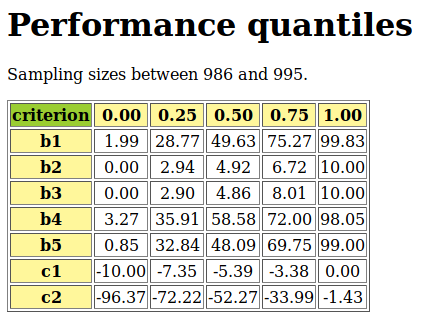
\includegraphics[width=7cm]{Figures/10-1-examplePerfQuantiles.png}
\caption[Showing updated quartiles limits per criterion]{\emph{Showing updated quartiles limits per criterion}. The $0.25$ column shows the first quartile (\texttt{Q1}) limits, the $0.50$ column shows the second quartile (\texttt{Q2}) limits and the $0.75$ column shows the third quartile (\texttt{Q3}) limits. Column $0.00$ (resp. $1.00$) shows the minimum (resp. maximum) performance on each criterion}
\label{fig:10.1}       % Give a unique label
\end{figure}
    
\section{Rating-by-ranking new performances with quantile norms}
\label{sec:10.3}

For \emph{rating} a newly given set of decision alternatives with the help of empirical performance quantiles estimated from historical data, the \texttt{sortingDigraphs} module provides the \texttt{Learned\-QuantilesRatingDigraph} class\index{LearnedQuantilesRatingDigraph@\texttt{LearnedQuantilesRatingDigraph} class}, a specialisation of the \texttt{QuantilesSor\-tingDigraph} class (see Chap.~\ref{sec:9}). The absolute rating result is computed by \emph{ranking} the new performance records together with the learned historical quantile limits.

The class constructor requires a valid \texttt{PerformanceQuantiles} instance and, by default, uses the \Copeland or the \NetFlows ranking rule, whichever fits best in an ordinal correlation sense with the underlying outranking digraph.

It is important to notice that the \texttt{LearnedQuantilesRatingDigraph} class, contrary to the generic \texttt{OutrankingDigraph} class, does not inherit from the generic \texttt{PerformanceTableau} class, but instead from the \texttt{Performance\-Quantiles} class \citep{BIS-2021b}.

The \texttt{actions} attribute in such a \texttt{LearnedQuantilesRatingDigraph} class instance contains not only the newly given decision alternatives, but also the historical quantile limits (attribute \texttt{profiles}) obtained from a given \texttt{Perfor\-manceQuantiles} class instance, i.e. estimated quantile bins' performance limits from historical performance data.

We reconsider now the \texttt{PerformanceQuantiles} object instance \texttt{pq} as computed in the previous section. Let \texttt{newActions} be a list of 10 new decision alternatives generated with the same random performance tableau generator \texttt{rpq} and including, for our didactical purpose, the two decision alternatives \texttt{a1001} and \texttt{a1010} mentioned at the beginning.
\begin{lstlisting}[caption={Computing the absolute rating of 10 new decision alternatives},label=list:10.4]
>>> from sortingDigraphs import LearnedQuantilesRatingDigraph
>>> newActions = rpg.randomActions(10)
>>> lqr = LearnedQuantilesRatingDigraph(pq,newActions,\
...                                     rankingRule='best')
>>> lqr
  *---- Object instance description
   Instance class      : LearnedQuantilesRatingDigraph
   Instance name       : normedRatingDigraph
   Criteria            : 7
   Quantile profiles   : 4
   Lower-closed bins   : True
   New actions         : 10
   Size                : 93
   Determinateness (%) : 76.1
   Ranking rule        : Copeland
   Ordinal correlation : +0.95
   Attributes: ['runTimes','objectives','criteria',
     'LowerClosed','quantilesFrequencies',
     'limitingQuantiles','historySizes','cdf','name',
     'newActions','evaluation','categories',
     'criteriaCategoryLimits','profiles','profileLimits',
     'hasNoVeto','actions','completeRelation','relation',
     'concordanceRelation','valuationdomain','order',
     'gamma','notGamma','rankingRule','rankingCorrelation',
     'rankingScores','actionsRanking','ratingCategories',
     'ratingRelation','relationOrig']
  *---- Constructor run times (in sec.)
   Threads           : 1
   Total time       : 0.02218
   Data input       : 0.00134
   Quantile classes : 0.00008
   Compute profiles : 0.00021
   Compute relation : 0.01869
   Compute rating   : 0.00186
   Compute sorting  : 0.00000
\end{lstlisting}

Data input to the \texttt{LearnedQuantilesRatingDigraph} class constructor are a valid \texttt{PerformanceQuantiles} object \texttt{pq} and a \texttt{newActions} list of newly generated decision alternatives with the same random generator \texttt{rpg} (see List.~\vref{list:10.4} Line 2-3).

The \texttt{actionsSubset} parameter of the \texttt{showPerformanceTableau()} method\index{showPerformanceTableau@\texttt{showPerformanceTableau()}} allows a look at the digraph's nodes, here called \texttt{newActions}.
\begin{lstlisting}[caption={Performance tableau of the new incoming decision alternatives},label=list:10.5,basicstyle=\ttfamily\scriptsize]
>>> lqr.showPerformanceTableau(actionsSubset=lqr.newActions)
 *----  performance tableau -----*
 criteria | a1001 a1002 a1003 a1004 a1005 a1006 a1007 a1008 a1009 a1010   
 ---------|-------------------------------------------------------------
    'b1'  |  37.0  27.0  24.0  16.0  42.0  33.0  39.0  64.0  42.0  32.0  
    'b2'  |   2.0   5.0   8.0   3.0   3.0   3.0   6.0   5.0   4.0   9.0  
    'b3'  |   2.0   4.0   2.0   1.0   6.0   3.0   2.0   6.0   6.0   6.0  
    'b4'  |  61.0  54.0  74.0  25.0  28.0  20.0  20.0  49.0  44.0  55.0  
    'b5'  |  31.0  63.0  61.0  48.0  30.0  39.0  16.0  96.0  57.0  51.0  
    'c1'  |  -4.0  -6.0  -8.0  -5.0  -1.0  -5.0  -1.0  -6.0  -6.0  -4.0  
    'c2'  | -40.0 -23.0 -37.0 -37.0 -24.0 -27.0 -73.0 -43.0 -94.0 -35.0  
\end{lstlisting}

Among the 10 new incoming decision alternatives, we recognise alternatives \texttt{a1001} (see column 2) and \texttt{a1010} (see last column) we have shown in Table~\vref{tab:10.1}.

The \texttt{actions} dictionary of a \texttt{LearnedQuantilesRatingDigraph} class instance includes, besides the 10 performance evaluations of the ten new alternatives, also the closed lower limits of the four quartile classes: \texttt{m1} = $[0.0- [$, \texttt{m2} = $[0.25- [$, \texttt{m3} = $[0.5- [$, \texttt{m4} = $[0.75 - [$. We find these limits in the \texttt{profiles} attribute (see List.~\vref{list:10.6} below).
\begin{lstlisting}[caption={Showing the limiting profiles of the rating quantiles},label=list:10.6]
>>> lqr.showPerformanceTableau(actionsSubset=lqr.profiles)
    *----  Quartiles limit profiles -----*
    criteria |  'm1'   'm2'   'm3'   'm4'   
    ---------|----------------------------
       'b1'  |  2.0    28.8   49.6   75.3  
       'b2'  |  0.0     2.9    4.9    6.7  
       'b3'  |  0.0     2.9    4.9    8.0  
       'b4'  |  3.3    35.9   58.6   72.0  
       'b5'  |  0.8    32.8   48.1   69.7  
       'c1'  | -10.0   -7.4   -5.4   -3.4  
       'c2'  | -96.4  -72.2  -52.3  -34.0  
\end{lstlisting}

The main run time is spent by the \texttt{LearnedQuantilesRatingDigraph} class constructor in computing a bipolar-valued outranking relation on the extended actions set including both the new alternatives as well as the quartile class limits (see List.~\vref{list:10.4} Lines 23-29).\footnote{In case of large volumes, i.e. many new decision alternatives and centile classes for instance, a multi-threading version may be used when multiple processing cores are available \citep{BIS-2021b}.}

The actual rating procedure will rely on a complete ranking of the new decision alternatives as well as the quantile class limits obtained from the corresponding bipolar-valued outranking digraph. Two efficient and scalable ranking rules, the \Copeland and its valued version, the \NetFlows rule may be used for this purpose. The \texttt{rankingRule} parameter allows to choose one of both. With \texttt{rankingRule='best'} (see List.~\vref{list:10.4} Line 3 ) the \texttt{LearnedQuantiles\-RatingDigraph} constructor will choose the ranking rule that results in the highest ordinal correlation with the given outranking relation (see Chap.~\ref{sec:22} and \citep{BIS-2012a}).

In this rating example, the \Copeland rule appears to be the more appropriate ranking rule.
\begin{lstlisting}[caption={\Copeland ranking of new alternatives and historical quartile limits},label=list:10.7]
>>> lqr.rankingRule
  'Copeland'
>>> lqr.actionsRanking
  ['m4', 'a1005', 'a1010', 'a1002', 'a1008', 'a1006', 'a1001',
   'a1003', 'm3', 'a1007', 'a1004', 'a1009', 'm2', 'm1'] 
>>> lqr.showCorrelation(lqr.rankingCorrelation)
  Correlation indexes:
    Crisp ordinal correlation  : +0.945
    Epistemic determination    :  0.522
    Bipolar-valued equivalence : +0.493
\end{lstlisting}

We achieve here in Listing.~\vref{list:10.7} a linear ranking without ties (from best to worst) of the digraph's actions set, i.e. including the new decision alternatives as well as the quartile limits $m1$ to $m4$, which is very close in an ordinal sense ($\tau = 0.945$) to the underlying strict outranking relation.

The eventual rating procedure is based in this example on the \emph{lower} quartile limits, such that the quartile classes' contents are filtered out in increasing order of the \emph{quartiles}.
\begin{lstlisting}
>>> lqr.ratingCategories
 OrderedDict([
 ('m2', ['a1007','a1004','a1009']),
 ('m3', ['a1005','a1010','a1002','a1008',
         'a1006','a1001','a1003'])
 ])
\end{lstlisting}    

We notice above that no new decision alternative is actually rated into the lowest $[0.0-0.25[$, respectively highest $[0.75- [$ quartile classes. Indeed, the absolute rating result is shown with the \texttt{showQuantilesRating()} method\index{showQuantilesRating@\texttt{showQuantilesRating()}}:
\begin{lstlisting}[caption={Absolute quartiles rating result},label=list:10.8]
>>> lqr.showQuantilesRating()
  *-------- Quartiles rating result ---------
   [0.50 - 0.75[ ['a1005', 'a1010', 'a1002', 'a1008',
                  'a1006', 'a1001', 'a1003']
   [0.25 - 0.50[ ['a1007', 'a1004', 'a1009']
\end{lstlisting}    

The same result may also be shown in a browser view with the \texttt{showHTMLRa\-tingHeatmap()} method\index{showHTMLRatingHeatmap@\texttt{showHTMLRatingHeatmap()}} using a specialised rating heatmap format (see Fig.~\vref{fig:10.2}): 
\begin{lstlisting}
>>> lqr.showHTMLRatingHeatmap(\
...            pageTitle='Heatmap of Quartiles Rating',\
...            Correlations=True,colorLevels=5)
\end{lstlisting}
\begin{figure}[ht]
\sidecaption[t]
 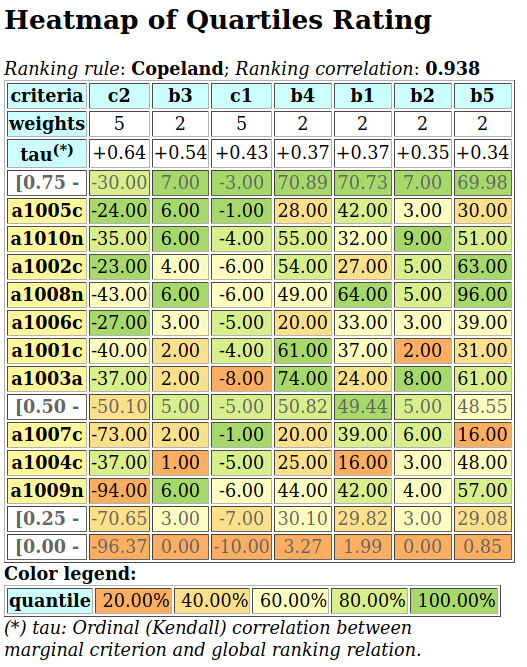
\includegraphics[width=7cm]{Figures/10-2-heatMap1.png}
\caption[Heatmap of absolute quartiles ranking]{\emph{Heatmap of absolute quartiles ranking}. The quartile equivalence classes appear lower-closed. No alternative is rated into the \texttt{Q1} class ($[0.00 - 0.25[$) and no alternative is rated into the Q4 class ($[0.75 - 1.00]$)}
\label{fig:10.2}       % Give a unique label
\end{figure}
	    
Using furthermore a specialised version of the \texttt{exportGraphViz()} method allows drawing in Figure~\vref{fig:10.3} the same rating result in a Hasse diagram format.\footnote{Note that the graphviz dot file was post-edited in order to mark in blue alternatives \texttt{a1001} and \texttt{a1010}.}
\begin{lstlisting}
>>> lqr.exportRatingGraphViz('quartileRatingDigraph')
 *---- exporting a dot file for GraphViz tools ---------*
  Exporting to quartileRatingDigraph.dot
  dot -Grankdir=TB -Tpng quartileRatingDigraph.dot -o quartileRatingDigraph.png
\end{lstlisting}
\begin{figure}[ht]
%\sidecaption[t]
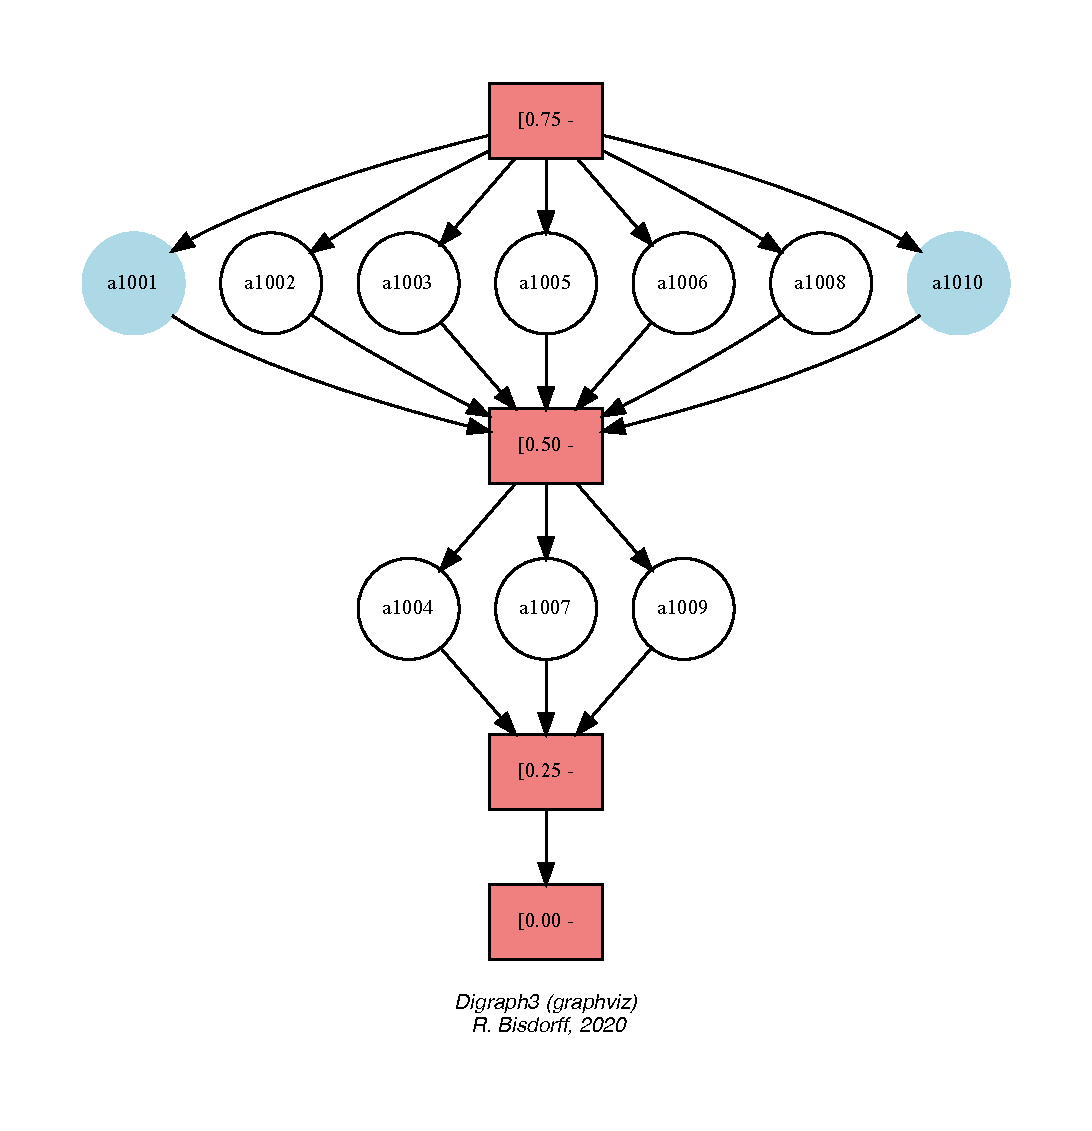
\includegraphics[width=\hsize]{Figures/10-3-normedRatingDigraph.pdf}
\caption{Absolute quartiles rating digraph}
\label{fig:10.3}       % Give a unique label
\end{figure}

We have actually solved now the \emph{absolute rating} problem stated at the beginning. Decision alternatives \texttt{a1001} and \texttt{a1010} (see Tab.~\vref{tab:10.1}) are both rated into the same third quartile \texttt{Q3} class (see Fig.~\vref{fig:10.3}), even if the \Copeland ranking, obtained from the underlying strict outranking digraph (see Fig.~\vref{fig:10.2}), suggests that alternative \texttt{a1010} is effectively \emph{better performing than} alternative \texttt{a1001}. 

A \emph{preciser} rating result may indeed be achieved when using \emph{deciles} instead of \emph{quartiles} for estimating the historical marginal cumulative distribution functions.
\begin{lstlisting}[caption={Absolute deciles rating result},label=list:10.9]
>>> pq1 = PerformanceQuantiles(pt, numberOfBins = 'deciles',\
...                 LowerClosed=True)
>>> pq1.updateQuantiles(newTab,historySize=None)
>>> lqr1 = LearnedQuantilesRatingDigraph(pq1,newActions,rankingRule='best')
>>> lqr1.showQuantilesRating()
  *-------- Deciles rating result ---------
   [0.60 - 0.70[ ['a1005', 'a1010', 'a1008', 'a1002']
   [0.50 - 0.60[ ['a1006', 'a1001', 'a1003']
   [0.40 - 0.50[ ['a1007', 'a1004']
   [0.30 - 0.40[ ['a1009']
\end{lstlisting}

Compared with the quartiles rating result, we notice in Listing~\vref{list:10.9} that the seven alternatives (\texttt{a1001}, \texttt{a1002}, \texttt{a1003}, \texttt{a1005}, \texttt{a1006}, \texttt{a1008} and \texttt{a1010}), rated before into the third quartile class $[0.50-0.75[$, are now divided up: alternatives \texttt{a1002}, \texttt{a1005}, \texttt{a1008} and \texttt{a1010} attain now the 7th decile class $[0.60-0.70[$, whereas alternatives \texttt{a1001}, \texttt{a1003} and \texttt{a1006} attain only the 6th decile class $[0.50-0.60[$. Of the three \texttt{Q2} $[0.25-0.50[$ rated alternatives (\texttt{a1004}, \texttt{a1007} and \texttt{a1009}), alternatives \texttt{a1004} and \texttt{a1007} are now rated into the 5th decile class $[0.40-0.50[$ and \texttt{a1009} is lowest rated into the 4th decile class $[0.30-0.40[$.

A browser heatmap view in Figure~\vref{fig:10.4} more conveniently illustrates this refined rating result.
\begin{lstlisting}
>>> lqr1.showHTMLRatingHeatmap(\
...       pageTitle='Heatmap of the deciles rating',\
...       colorLevels=5, Correlations=True)
\end{lstlisting}
\begin{figure}[ht]
\sidecaption[t]
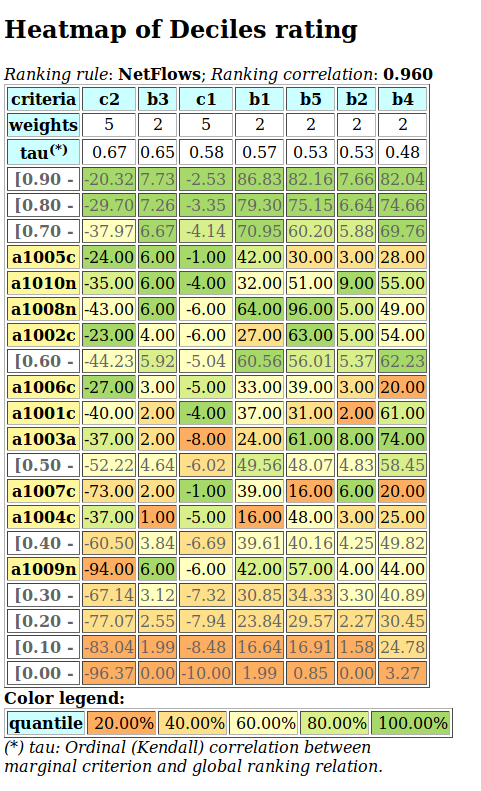
\includegraphics[width=7cm]{Figures/10-4-heatMap2.png}
\caption[Heatmap of absolute deciles rating]{\emph{Heatmap of absolute deciles rating}. Decision alternatives \texttt{a1001} and \texttt{a1010} are now, as expected, rated in the $6^{th}$ decile (\texttt{D6}), respectively in the $7^{th}$ decile (\texttt{D7})}
\label{fig:10.4}       % Give a unique label
\end{figure}

To avoid having to recompute performance deciles from historical data when wishing to refine a rating result, it is useful, depending on the actual size of the historical data, to initially compute performance quantiles with a relatively high number of bins, for instance \emph{dodeciles} or even \emph{centiles}. It is then possible to interpolate on the fly \emph{quartiles} or \emph{deciles} for instance, when constructing the rating digraph. 
\begin{lstlisting}[caption={From deciles interpolated quartiles rating result},label=list:10.10]
>>> lqr2 = LearnedQuantilesRatingDigraph(pq1,newActions,
...                   quantiles='quartiles')
>>> lqr2.showQuantilesRating()
  *-------- Deciles rating result ---------
   [0.50 - 0.75[ ['a1005', 'a1010', 'a1002', 'a1008',
                  'a1006', 'a1001', 'a1003']
   [0.25 - 0.50[ ['a1004', 'a1007', 'a1009']
\end{lstlisting}

With the \texttt{quantiles} parameter (see List.~\vref{list:10.10} Line 2), we recover by interpolation the same quartiles rating as obtained directly with historical performance quartiles (see List.~\vref{list:10.8}). Mind that a correct interpolation of quantiles from a given cumulative distribution function requires more or less uniform distributions of observations in each bin. 
More generally, in the case of industrial production monitoring problems, for instance, where large volumes of historical performance data may be available, it can be of interest to estimate even more precisely the marginal cumulative distribution functions, especially when \emph{tail} rating results, i.e. distinguishing \emph{very best}, or \emph{very weak} multiple-criteria performances, become a critical issue. Similarly, the \texttt{historySize} parameter may be used for monitoring on the fly \emph{unstable} random multiple-criteria performance data \citep{CHAM-2006}.  	

%%%%%%%
%The chapter bibliography
%\normallatexbib
%\clearpage
%\phantomsection
%\addcontentsline{toc}{section}{References}
%\chapter{Rating by ranking with learned performance quantile norms}
\label{sec:10}

\abstract*{ We address in Chapter~\ref{sec:10} the problem of rating multiple-criteria performances of a set of potential decision alternatives with respect to performance quantiles learned from historical performance data gathered from similar decision alternatives observed in the past. We show how to learn performance quantiles from historical performance tableaux. New performance records may now be rated with respect to these quantile norms.}

\abstract{ We address in Chapter~\ref{sec:10} the problem of rating multiple-criteria performances of a set of potential decision alternatives with respect to performance quantiles learned from historical performance data gathered from similar decision alternatives observed in the past. We show how to learn performance quantiles from historical performance tableaux. New performance records may now be rated with respect to these quantile norms.}

\section{The absolute rating problem}
\label{sec:10.1}
	  
To illustrate the \emph{absolute rating} problem we face, consider for a moment that, in a given decision making problem we observe, for instance, in Table~\vref{tab:10.1} below, the multi-criteria performance evaluations of two potential decision alternatives, named \texttt{a1001} and \texttt{a1010}, evaluated on 7 \emph{incommensurable} performance criteria: 2 \emph{Costs} criteria \texttt{c1} and \texttt{c2} (to \emph{minimise}) and 5 \emph{Benefits} criteria \texttt{b1} to \texttt{b5} (to \emph{maximise}). 
\begin{table}[ht]
\caption{Multi-criteria performances of two potential decision alternatives}
\label{tab:10.1}       % Give a unique label
\begin{center}
  %\begin{small}
    \begin{tabular}{l|c|c|c|c|c|c|c}
      \svhline\noalign{\smallskip}
      Criterion (weight) & \texttt{b1} (2) & \texttt{b2} (2) & \texttt{b3} (2) & \texttt{b4} (2) & \texttt{b5} (2) & \texttt{c1} (5) & \texttt{c2} (5)\\
      \noalign{\smallskip}\hline\noalign{\smallskip}
    \texttt{a1001} &   37.0  &  2 & 2 & 61.0 & 31.0 & -4 & -40.0\\
    \texttt{a1010} &   32.0 & 9 & 6 & 55.0 & 51.0 & -4 & -35.0 \\
      \noalign{\smallskip}\hline
    \end{tabular}
  %\end{small}
\end{center}
\end{table}

The performance on \emph{Benefits} criteria \texttt{b1}, \texttt{b4} and \texttt{b5} is measured on a cardinal scale from $0.0$ (worst) to $100.0$ (best) whereas, the performance on the \emph{Benefits} criteria \texttt{b2} and \texttt{b3}  and on the \emph{Costs} criterion \texttt{c1} is measured on an ordinal scale from $0$ (worst) to $10$ (best), respectively $-10$ (worst) to $0$ (best). The performance on the \emph{Costs} criterion \texttt{c2} is eventually measured on a cardinal \emph{negative} scale from $-100.00$ (worst) to $0.0$ (best). The two \emph{Costs} criteria are equi-significant (weight 5). Similarly, the five Benefits criteria are also equi-significant (weight 2). The \emph{importance} (sum of significance weights: $2 \times 5 = 10$) of the \emph{Costs} criteria is hence \emph{equivalent} to the \emph{importance} (sum of significance weights: $5 \times 2 = 10$) of the \emph{Benefits} criteria.
   
The non trivial decision problem we now face, is to decide, how the previous two multiple-criteria performance records of alternatives \texttt{a1001}, respectively \texttt{a1010},  may be rated: \emph{excellent}~? \emph{good}~?, or \emph{fair}~?; perhaps even, \emph{weak}~? or \emph{very weak}~? when compared with similar multi-criteria performance records one has already rated into quantiles in the past. 

To solve this \emph{absolute} rating problem, first, we need to estimate multi-criteria \emph{performance quantiles} from historical records \citep{CPSTAT-L5}.  

\section{Incremental learning of historical performance quantiles}
\label{sec:10.2}

Suppose that we see flying in random multiple-criteria performances from a given model of random performance tableau (see Chap.~\ref{sec:5}). The question we address here is to estimate empirical performance quantiles on the basis of so far observed performance vectors. For this task, we are inspired by \citet*{CHAM-2006}, who present an efficient algorithm for incrementally updating a quantile-binned cumulative distribution function (CDF) with newly observed CDFs\footnote{We have adapted in Python a C++ implementation published by \citep*[Chapter 5]{NR3-2007}.}. 

The \texttt{PerformanceQuantiles}\index{PerformanceQuantiles@\texttt{PerformanceQuantiles} class} class, using the \texttt{IncrementalQuan\-tiles\-Estimator} class\index{IncrementalQuantilesEstimator@\texttt{IncrementalQuantilesEstimator} class} from the \texttt{randomNumbers} module \index{randomNumbers@\texttt{randomNumbers} module}, implements such a performance quantiles estimation based on a given performance tableau \citep{BIS-2021b}.

Its main attributes are:
\begin{itemize}[rightmargin=0.5cm,leftmargin=0.5cm,topsep=1pt]
\item Ordered \texttt{objectives} and a \texttt{criteria} dictionaries from a valid performance tableau instance;
\item A list \texttt{quantileFrequencies} of quantile frequencies like:
  \begin{itemize}[nosep]
  \item \emph{quartiles} $[0.0, 0.25, 05, 0.75,1.0]$,
  \item  \emph{quintiles} $[0.0, 0.2, 0.4, 0.6, 0.8, 1.0]$ or
  \item  \emph{deciles} $[0.0, 0.1, 0.2, ... 1.0]$ for instance;
  \end{itemize}
\item An ordered  dictionary \texttt{limitingQuantiles} of so far estimated \emph{lower} (default) or \emph{upper} quantile class limits for each frequency per criterion;
\item An ordered dictionary \texttt{historySizes} for keeping track of the number of evaluations seen so far per criterion. Missing data, the case given, make these sizes vary from criterion to criterion.
\end{itemize}

Below, we show an example Python session concerning 900 decision alternatives randomly generated with a \emph{Cost-Benefit} performance tableau model (see Sec.~\ref{sec:5.3}) from which are also drawn the performances of alternatives \texttt{a1001} and \texttt{a1010} shown in Table~\vref{tab:10.1} above.
\begin{lstlisting}[caption={Computing performance quantiles from a given performance tableau},label=list:10.1]
>>> from performanceQuantiles import PerformanceQuantiles
>>> from randomPerfTabs import RandomCBPerformanceTableau
>>> nbrActions=900
>>> nbrCrit = 7
>>> seed = 100
>>> pt = RandomCBPerformanceTableau(numberOfActions=nbrActions,\
...                  numberOfCriteria=nbrCrit,seed=seed)
>>> pq = PerformanceQuantiles(pt,\
...                   numberOfBins = 'quartiles',\
...                   LowerClosed=True)
>>> pq
  *------- PerformanceQuantiles instance description ------*
   Instance class   : PerformanceQuantiles
   Instance name    : 4-tiled_performances
   Objectives       : 2
   Criteria         : 7
   Quantiles        : 4
   History sizes    : {'c1': 887,'b1': 888,'b2': 891,'b3': 895,
                        'b4': 892,'c2': 893,'b5': 887}
   Attributes       : ['perfTabType','valueDigits',
                       'actionsTypeStatistics',
                       'objectives', 'BigData',
                       'missingDataProbability',
		       'criteria', 'LowerClosed', 'name',
		       'quantilesFrequencies', 'historySizes',
		       'limitingQuantiles', 'cdf']
\end{lstlisting}
The \texttt{PerformanceQuantiles} class parameter \texttt{numberOfBins} (see List.~\vref{list:10.1} Line 9 above), choosing the wished number of quantile frequencies, may be either \emph{quartiles} (4 bins), \emph{quintiles} (5 bins), \emph{deciles} (10 bins), \emph{dodeciles} (20 bins) or any other integer number of quantile bins. The quantile bins may be either \emph{lower closed} (default) or \emph{upper-closed}.

Inspecting the estimated quartile limits may be operated with the\\ \texttt{showLimitingQuantiles()} method.\index{showLimitingQuantiles@\texttt{showLimitingQuantiles()}}
\begin{lstlisting}[caption={Printing out the estimated quartile limits},label=list:10.2]
>>> pq.showLimitingQuantiles(ByObjectives=True)
    ----  Historical performance quantiles -----*
    Costs
    criteria | weights |  '0.00' '0.25' '0.50' '0.75' '1.00'   
    ---------|----------------------------------------------------
       'c1'  |    5    |   -10    -7     -5     -3      0  
       'c2'  |    5    | -96.37 -70.65 -50.10 -30.00  -1.43  
    Benefits
    criteria | weights | '0.00'  '0.25' '0.50' '0.75' '1.00'   
    ---------|-----------------------------------------------------
       'b1'  |    2    |  1.99    29.82 49.44  70.73  99.83  
       'b2'  |    2    |    0      3      5      7     10  
       'b3'  |    2    |    0      3      5      7     10  
       'b4'  |    2    |  3.27   30.10  50.82  70.89  98.05  
       'b5'  |    2    |  0.85   29.08  48.55  69.98  97.56  
\end{lstlisting}
Both objectives are \emph{equally important}; the sum of weights (10) of the \emph{Costs} criteria balance the sum of weights (10) of the \emph{Benefits} criteria (see List.~\vref{list:10.2} column 2). The preference direction of the \emph{Costs} criteria \texttt{c1} and \texttt{c2} is \emph{negative}; the lesser the costs, the better it is, whereas all the \emph{Benefits} criteria \texttt{b1} to \texttt{b5} show \emph{positive} preference directions, i.e. the higher the benefits, the better it is. The columns entitled '$0.00$', resp. '$1.00$' show the \emph{quartile} \texttt{Q0}, resp. \texttt{Q4}, i.e. the \emph{worst}, resp. \emph{best} performance observed so far on each criterion. Column '$0.50$' shows the \emph{median} (\texttt{Q2}) performance observed on the criteria.  

New  decision alternatives with random multiple-criteria performance vectors from the same random performance tableau model as \texttt{pt} (see List.~\vref{list:10.1}) may now be generated with a generic \texttt{RandomPerformanceGenerator} class\index{RandomPerformanceGenerator@\texttt{RandomPerformanceGenerator()}} from the \texttt{randomPerfTabs} module \citep{BIS-2021b}.\footnote{The \texttt{RandomPerformanceGenerator} class works for the \emph{standard} performance tableau model (see Sec.~\ref{sec:5.2}), the \emph{Cost-Benefit} model (see Sec.~\ref{sec:5.3}), and the 3-objectives model (see Sec.~\ref{sec:5.4}).}
\begin{lstlisting}[caption={Generating 100 new random decision alternatives of the same model},label=list:10.3]
>>> from randomPerfTabs import RandomPerformanceGenerator
>>> rpg = RandomPerformanceGenerator(tp,seed=seed)
>>> newTab = rpg.randomPerformanceTableau(100)
\end{lstlisting}

The so far estimated historical quantile limits must, first, be updated with this newly arriving 100 data records:
\begin{lstlisting}
>>> # Updating the quartile norms shown above 
>>> pq.updateQuantiles(newTab,historySize=None)
\end{lstlisting}
Parameter \texttt{historySize} of the \texttt{updateQuantiles()} method\index{updateQuantiles@\texttt{updateQuantiles()}} (Line 2 above) allows to \emph{balance} the \emph{new} evaluations against the \emph{historical} ones.

With \texttt{historySize = None} (the default setting), the balance in the example above is $900/1000$ ($90\%$, the weight of historical data) against $100/1000$ ($10\%$, the weight of the new incoming observations). Setting \texttt{historySize = 0}, for instance, will ignore all historical data ($0/100$ against $100/100$) and restart building the quantile estimation with solely the new incoming data. The \texttt{showHTMLLimitingQuantiles()} method\index{showHTMLLimitingQuantiles@\texttt{showHTMLLimitingQuantiles()}} shows the updated quantile limits in a browser view (see Fig.~\vref{fig:10.1}).
\begin{lstlisting}
>>> # showing the updated quantile limits in a browser view
>>> pq.showHTMLLimitingQuantiles(Transposed=True)
\end{lstlisting}
\begin{figure}[ht]
\sidecaption[t]
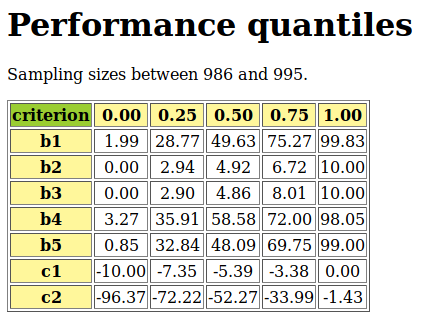
\includegraphics[width=7cm]{Figures/10-1-examplePerfQuantiles.png}
\caption[Showing updated quartiles limits per criterion]{\emph{Showing updated quartiles limits per criterion}. The $0.25$ column shows the first quartile (\texttt{Q1}) limits, the $0.50$ column shows the second quartile (\texttt{Q2}) limits and the $0.75$ column shows the third quartile (\texttt{Q3}) limits. Column $0.00$ (resp. $1.00$) shows the minimum (resp. maximum) performance on each criterion}
\label{fig:10.1}       % Give a unique label
\end{figure}
    
\section{Rating-by-ranking new performances with quantile norms}
\label{sec:10.3}

For \emph{rating} a newly given set of decision alternatives with the help of empirical performance quantiles estimated from historical data, the \texttt{sortingDigraphs} module provides the \texttt{Learned\-QuantilesRatingDigraph} class\index{LearnedQuantilesRatingDigraph@\texttt{LearnedQuantilesRatingDigraph} class}, a specialisation of the \texttt{QuantilesSor\-tingDigraph} class (see Chap.~\ref{sec:9}). The absolute rating result is computed by \emph{ranking} the new performance records together with the learned historical quantile limits.

The class constructor requires a valid \texttt{PerformanceQuantiles} instance and, by default, uses the \Copeland or the \NetFlows ranking rule, whichever fits best in an ordinal correlation sense with the underlying outranking digraph.

It is important to notice that the \texttt{LearnedQuantilesRatingDigraph} class, contrary to the generic \texttt{OutrankingDigraph} class, does not inherit from the generic \texttt{PerformanceTableau} class, but instead from the \texttt{Performance\-Quantiles} class \citep{BIS-2021b}.

The \texttt{actions} attribute in such a \texttt{LearnedQuantilesRatingDigraph} class instance contains not only the newly given decision alternatives, but also the historical quantile limits (attribute \texttt{profiles}) obtained from a given \texttt{Perfor\-manceQuantiles} class instance, i.e. estimated quantile bins' performance limits from historical performance data.

We reconsider now the \texttt{PerformanceQuantiles} object instance \texttt{pq} as computed in the previous section. Let \texttt{newActions} be a list of 10 new decision alternatives generated with the same random performance tableau generator \texttt{rpq} and including, for our didactical purpose, the two decision alternatives \texttt{a1001} and \texttt{a1010} mentioned at the beginning.
\begin{lstlisting}[caption={Computing the absolute rating of 10 new decision alternatives},label=list:10.4]
>>> from sortingDigraphs import LearnedQuantilesRatingDigraph
>>> newActions = rpg.randomActions(10)
>>> lqr = LearnedQuantilesRatingDigraph(pq,newActions,\
...                                     rankingRule='best')
>>> lqr
  *---- Object instance description
   Instance class      : LearnedQuantilesRatingDigraph
   Instance name       : normedRatingDigraph
   Criteria            : 7
   Quantile profiles   : 4
   Lower-closed bins   : True
   New actions         : 10
   Size                : 93
   Determinateness (%) : 76.1
   Ranking rule        : Copeland
   Ordinal correlation : +0.95
   Attributes: ['runTimes','objectives','criteria',
     'LowerClosed','quantilesFrequencies',
     'limitingQuantiles','historySizes','cdf','name',
     'newActions','evaluation','categories',
     'criteriaCategoryLimits','profiles','profileLimits',
     'hasNoVeto','actions','completeRelation','relation',
     'concordanceRelation','valuationdomain','order',
     'gamma','notGamma','rankingRule','rankingCorrelation',
     'rankingScores','actionsRanking','ratingCategories',
     'ratingRelation','relationOrig']
  *---- Constructor run times (in sec.)
   Threads           : 1
   Total time       : 0.02218
   Data input       : 0.00134
   Quantile classes : 0.00008
   Compute profiles : 0.00021
   Compute relation : 0.01869
   Compute rating   : 0.00186
   Compute sorting  : 0.00000
\end{lstlisting}

Data input to the \texttt{LearnedQuantilesRatingDigraph} class constructor are a valid \texttt{PerformanceQuantiles} object \texttt{pq} and a \texttt{newActions} list of newly generated decision alternatives with the same random generator \texttt{rpg} (see List.~\vref{list:10.4} Line 2-3).

The \texttt{actionsSubset} parameter of the \texttt{showPerformanceTableau()} method\index{showPerformanceTableau@\texttt{showPerformanceTableau()}} allows a look at the digraph's nodes, here called \texttt{newActions}.
\begin{lstlisting}[caption={Performance tableau of the new incoming decision alternatives},label=list:10.5,basicstyle=\ttfamily\scriptsize]
>>> lqr.showPerformanceTableau(actionsSubset=lqr.newActions)
 *----  performance tableau -----*
 criteria | a1001 a1002 a1003 a1004 a1005 a1006 a1007 a1008 a1009 a1010   
 ---------|-------------------------------------------------------------
    'b1'  |  37.0  27.0  24.0  16.0  42.0  33.0  39.0  64.0  42.0  32.0  
    'b2'  |   2.0   5.0   8.0   3.0   3.0   3.0   6.0   5.0   4.0   9.0  
    'b3'  |   2.0   4.0   2.0   1.0   6.0   3.0   2.0   6.0   6.0   6.0  
    'b4'  |  61.0  54.0  74.0  25.0  28.0  20.0  20.0  49.0  44.0  55.0  
    'b5'  |  31.0  63.0  61.0  48.0  30.0  39.0  16.0  96.0  57.0  51.0  
    'c1'  |  -4.0  -6.0  -8.0  -5.0  -1.0  -5.0  -1.0  -6.0  -6.0  -4.0  
    'c2'  | -40.0 -23.0 -37.0 -37.0 -24.0 -27.0 -73.0 -43.0 -94.0 -35.0  
\end{lstlisting}

Among the 10 new incoming decision alternatives, we recognise alternatives \texttt{a1001} (see column 2) and \texttt{a1010} (see last column) we have shown in Table~\vref{tab:10.1}.

The \texttt{actions} dictionary of a \texttt{LearnedQuantilesRatingDigraph} class instance includes, besides the 10 performance evaluations of the ten new alternatives, also the closed lower limits of the four quartile classes: \texttt{m1} = $[0.0- [$, \texttt{m2} = $[0.25- [$, \texttt{m3} = $[0.5- [$, \texttt{m4} = $[0.75 - [$. We find these limits in the \texttt{profiles} attribute (see List.~\vref{list:10.6} below).
\begin{lstlisting}[caption={Showing the limiting profiles of the rating quantiles},label=list:10.6]
>>> lqr.showPerformanceTableau(actionsSubset=lqr.profiles)
    *----  Quartiles limit profiles -----*
    criteria |  'm1'   'm2'   'm3'   'm4'   
    ---------|----------------------------
       'b1'  |  2.0    28.8   49.6   75.3  
       'b2'  |  0.0     2.9    4.9    6.7  
       'b3'  |  0.0     2.9    4.9    8.0  
       'b4'  |  3.3    35.9   58.6   72.0  
       'b5'  |  0.8    32.8   48.1   69.7  
       'c1'  | -10.0   -7.4   -5.4   -3.4  
       'c2'  | -96.4  -72.2  -52.3  -34.0  
\end{lstlisting}

The main run time is spent by the \texttt{LearnedQuantilesRatingDigraph} class constructor in computing a bipolar-valued outranking relation on the extended actions set including both the new alternatives as well as the quartile class limits (see List.~\vref{list:10.4} Lines 23-29).\footnote{In case of large volumes, i.e. many new decision alternatives and centile classes for instance, a multi-threading version may be used when multiple processing cores are available \citep{BIS-2021b}.}

The actual rating procedure will rely on a complete ranking of the new decision alternatives as well as the quantile class limits obtained from the corresponding bipolar-valued outranking digraph. Two efficient and scalable ranking rules, the \Copeland and its valued version, the \NetFlows rule may be used for this purpose. The \texttt{rankingRule} parameter allows to choose one of both. With \texttt{rankingRule='best'} (see List.~\vref{list:10.4} Line 3 ) the \texttt{LearnedQuantiles\-RatingDigraph} constructor will choose the ranking rule that results in the highest ordinal correlation with the given outranking relation (see Chap.~\ref{sec:22} and \citep{BIS-2012a}).

In this rating example, the \Copeland rule appears to be the more appropriate ranking rule.
\begin{lstlisting}[caption={\Copeland ranking of new alternatives and historical quartile limits},label=list:10.7]
>>> lqr.rankingRule
  'Copeland'
>>> lqr.actionsRanking
  ['m4', 'a1005', 'a1010', 'a1002', 'a1008', 'a1006', 'a1001',
   'a1003', 'm3', 'a1007', 'a1004', 'a1009', 'm2', 'm1'] 
>>> lqr.showCorrelation(lqr.rankingCorrelation)
  Correlation indexes:
    Crisp ordinal correlation  : +0.945
    Epistemic determination    :  0.522
    Bipolar-valued equivalence : +0.493
\end{lstlisting}

We achieve here in Listing.~\vref{list:10.7} a linear ranking without ties (from best to worst) of the digraph's actions set, i.e. including the new decision alternatives as well as the quartile limits $m1$ to $m4$, which is very close in an ordinal sense ($\tau = 0.945$) to the underlying strict outranking relation.

The eventual rating procedure is based in this example on the \emph{lower} quartile limits, such that the quartile classes' contents are filtered out in increasing order of the \emph{quartiles}.
\begin{lstlisting}
>>> lqr.ratingCategories
 OrderedDict([
 ('m2', ['a1007','a1004','a1009']),
 ('m3', ['a1005','a1010','a1002','a1008',
         'a1006','a1001','a1003'])
 ])
\end{lstlisting}    

We notice above that no new decision alternative is actually rated into the lowest $[0.0-0.25[$, respectively highest $[0.75- [$ quartile classes. Indeed, the absolute rating result is shown with the \texttt{showQuantilesRating()} method\index{showQuantilesRating@\texttt{showQuantilesRating()}}:
\begin{lstlisting}[caption={Absolute quartiles rating result},label=list:10.8]
>>> lqr.showQuantilesRating()
  *-------- Quartiles rating result ---------
   [0.50 - 0.75[ ['a1005', 'a1010', 'a1002', 'a1008',
                  'a1006', 'a1001', 'a1003']
   [0.25 - 0.50[ ['a1007', 'a1004', 'a1009']
\end{lstlisting}    

The same result may also be shown in a browser view with the \texttt{showHTMLRa\-tingHeatmap()} method\index{showHTMLRatingHeatmap@\texttt{showHTMLRatingHeatmap()}} using a specialised rating heatmap format (see Fig.~\vref{fig:10.2}): 
\begin{lstlisting}
>>> lqr.showHTMLRatingHeatmap(\
...            pageTitle='Heatmap of Quartiles Rating',\
...            Correlations=True,colorLevels=5)
\end{lstlisting}
\begin{figure}[ht]
\sidecaption[t]
 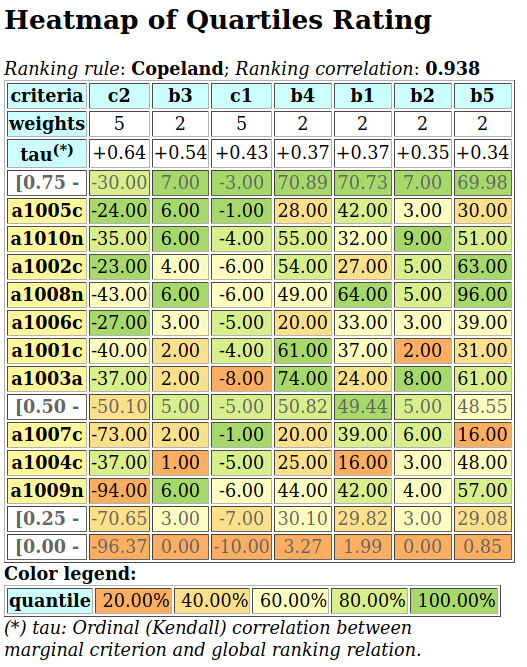
\includegraphics[width=7cm]{Figures/10-2-heatMap1.png}
\caption[Heatmap of absolute quartiles ranking]{\emph{Heatmap of absolute quartiles ranking}. The quartile equivalence classes appear lower-closed. No alternative is rated into the \texttt{Q1} class ($[0.00 - 0.25[$) and no alternative is rated into the Q4 class ($[0.75 - 1.00]$)}
\label{fig:10.2}       % Give a unique label
\end{figure}
	    
Using furthermore a specialised version of the \texttt{exportGraphViz()} method allows drawing in Figure~\vref{fig:10.3} the same rating result in a Hasse diagram format.\footnote{Note that the graphviz dot file was post-edited in order to mark in blue alternatives \texttt{a1001} and \texttt{a1010}.}
\begin{lstlisting}
>>> lqr.exportRatingGraphViz('quartileRatingDigraph')
 *---- exporting a dot file for GraphViz tools ---------*
  Exporting to quartileRatingDigraph.dot
  dot -Grankdir=TB -Tpng quartileRatingDigraph.dot -o quartileRatingDigraph.png
\end{lstlisting}
\begin{figure}[ht]
%\sidecaption[t]
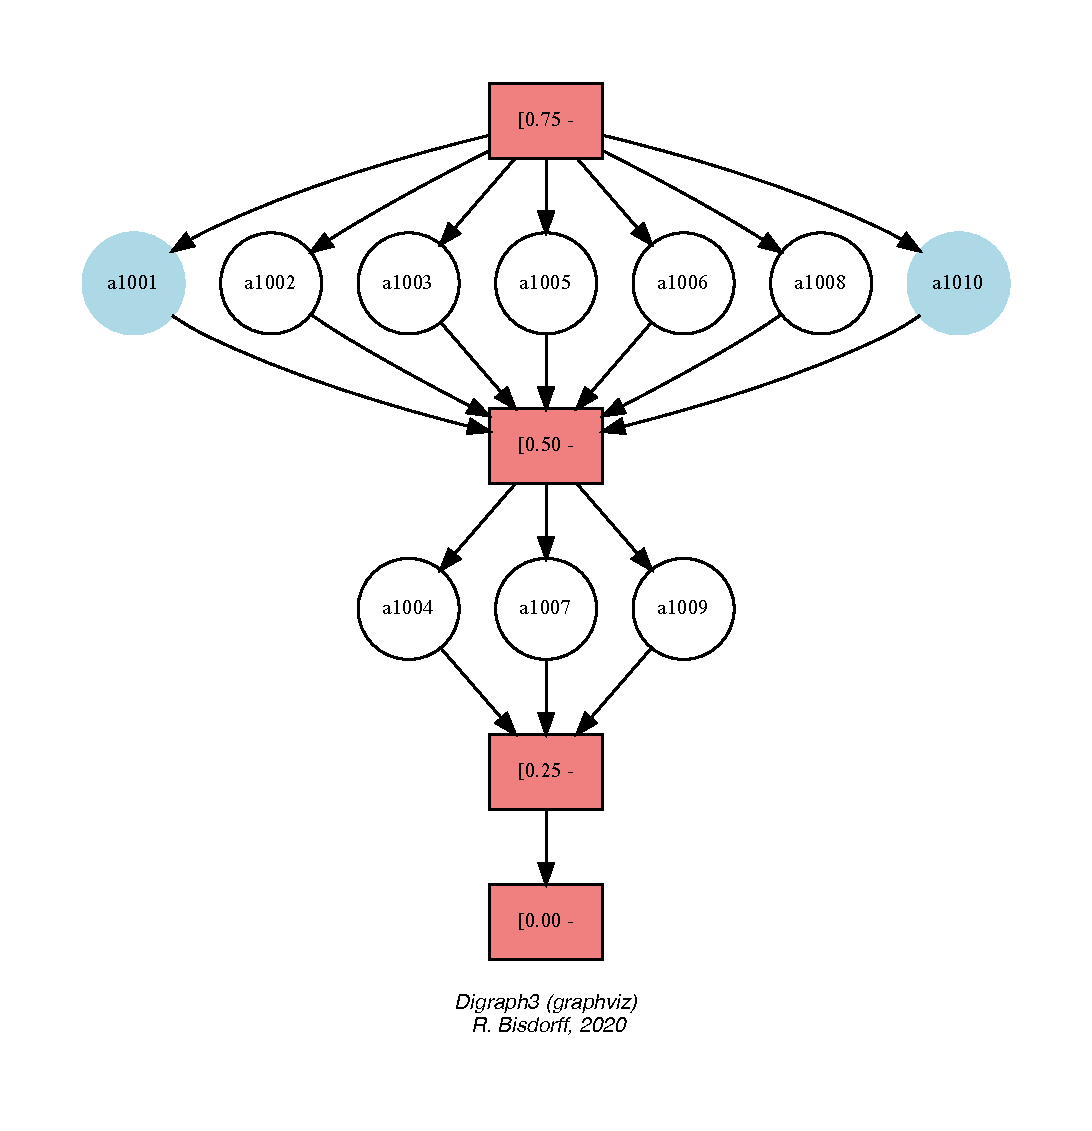
\includegraphics[width=\hsize]{Figures/10-3-normedRatingDigraph.pdf}
\caption{Absolute quartiles rating digraph}
\label{fig:10.3}       % Give a unique label
\end{figure}

We have actually solved now the \emph{absolute rating} problem stated at the beginning. Decision alternatives \texttt{a1001} and \texttt{a1010} (see Tab.~\vref{tab:10.1}) are both rated into the same third quartile \texttt{Q3} class (see Fig.~\vref{fig:10.3}), even if the \Copeland ranking, obtained from the underlying strict outranking digraph (see Fig.~\vref{fig:10.2}), suggests that alternative \texttt{a1010} is effectively \emph{better performing than} alternative \texttt{a1001}. 

A \emph{preciser} rating result may indeed be achieved when using \emph{deciles} instead of \emph{quartiles} for estimating the historical marginal cumulative distribution functions.
\begin{lstlisting}[caption={Absolute deciles rating result},label=list:10.9]
>>> pq1 = PerformanceQuantiles(pt, numberOfBins = 'deciles',\
...                 LowerClosed=True)
>>> pq1.updateQuantiles(newTab,historySize=None)
>>> lqr1 = LearnedQuantilesRatingDigraph(pq1,newActions,rankingRule='best')
>>> lqr1.showQuantilesRating()
  *-------- Deciles rating result ---------
   [0.60 - 0.70[ ['a1005', 'a1010', 'a1008', 'a1002']
   [0.50 - 0.60[ ['a1006', 'a1001', 'a1003']
   [0.40 - 0.50[ ['a1007', 'a1004']
   [0.30 - 0.40[ ['a1009']
\end{lstlisting}

Compared with the quartiles rating result, we notice in Listing~\vref{list:10.9} that the seven alternatives (\texttt{a1001}, \texttt{a1002}, \texttt{a1003}, \texttt{a1005}, \texttt{a1006}, \texttt{a1008} and \texttt{a1010}), rated before into the third quartile class $[0.50-0.75[$, are now divided up: alternatives \texttt{a1002}, \texttt{a1005}, \texttt{a1008} and \texttt{a1010} attain now the 7th decile class $[0.60-0.70[$, whereas alternatives \texttt{a1001}, \texttt{a1003} and \texttt{a1006} attain only the 6th decile class $[0.50-0.60[$. Of the three \texttt{Q2} $[0.25-0.50[$ rated alternatives (\texttt{a1004}, \texttt{a1007} and \texttt{a1009}), alternatives \texttt{a1004} and \texttt{a1007} are now rated into the 5th decile class $[0.40-0.50[$ and \texttt{a1009} is lowest rated into the 4th decile class $[0.30-0.40[$.

A browser heatmap view in Figure~\vref{fig:10.4} more conveniently illustrates this refined rating result.
\begin{lstlisting}
>>> lqr1.showHTMLRatingHeatmap(\
...       pageTitle='Heatmap of the deciles rating',\
...       colorLevels=5, Correlations=True)
\end{lstlisting}
\begin{figure}[ht]
\sidecaption[t]
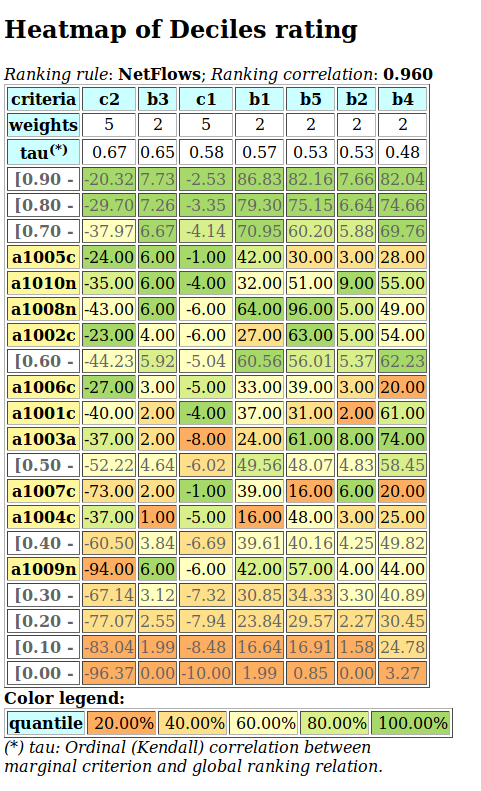
\includegraphics[width=7cm]{Figures/10-4-heatMap2.png}
\caption[Heatmap of absolute deciles rating]{\emph{Heatmap of absolute deciles rating}. Decision alternatives \texttt{a1001} and \texttt{a1010} are now, as expected, rated in the $6^{th}$ decile (\texttt{D6}), respectively in the $7^{th}$ decile (\texttt{D7})}
\label{fig:10.4}       % Give a unique label
\end{figure}

To avoid having to recompute performance deciles from historical data when wishing to refine a rating result, it is useful, depending on the actual size of the historical data, to initially compute performance quantiles with a relatively high number of bins, for instance \emph{dodeciles} or even \emph{centiles}. It is then possible to interpolate on the fly \emph{quartiles} or \emph{deciles} for instance, when constructing the rating digraph. 
\begin{lstlisting}[caption={From deciles interpolated quartiles rating result},label=list:10.10]
>>> lqr2 = LearnedQuantilesRatingDigraph(pq1,newActions,
...                   quantiles='quartiles')
>>> lqr2.showQuantilesRating()
  *-------- Deciles rating result ---------
   [0.50 - 0.75[ ['a1005', 'a1010', 'a1002', 'a1008',
                  'a1006', 'a1001', 'a1003']
   [0.25 - 0.50[ ['a1004', 'a1007', 'a1009']
\end{lstlisting}

With the \texttt{quantiles} parameter (see List.~\vref{list:10.10} Line 2), we recover by interpolation the same quartiles rating as obtained directly with historical performance quartiles (see List.~\vref{list:10.8}). Mind that a correct interpolation of quantiles from a given cumulative distribution function requires more or less uniform distributions of observations in each bin. 
More generally, in the case of industrial production monitoring problems, for instance, where large volumes of historical performance data may be available, it can be of interest to estimate even more precisely the marginal cumulative distribution functions, especially when \emph{tail} rating results, i.e. distinguishing \emph{very best}, or \emph{very weak} multiple-criteria performances, become a critical issue. Similarly, the \texttt{historySize} parameter may be used for monitoring on the fly \emph{unstable} random multiple-criteria performance data \citep{CHAM-2006}.  	

%%%%%%%
%The chapter bibliography
%\normallatexbib
%\clearpage
%\phantomsection
%\addcontentsline{toc}{section}{References}
%\input{02-mainMatters/10-chapterAbsoluteRating.bbl} 
\bibliographystyle{spbasic}
\bibliography{03-backMatters/reference}
 
\bibliographystyle{spbasic}
\bibliography{03-backMatters/reference}
 
\bibliographystyle{spbasic}
\bibliography{03-backMatters/reference}
 
